\documentclass[xcolor=svgnames,9pt,english,aspectratio=169,t]{beamer}
%\documentclass[xcolor=svgnames,9pt,english,handout,aspectratio=169,t]{beamer}
\newcommand{\handout}{0}

% =====================================================================
% POLI 450A (2026) --- shared TEMPLATE layer.
%
% Input from each lecture near the top of its file, BEFORE
% ../course_theme.tex (metropolis must be selected before the course
% palette overrides it):
%
%   \documentclass[xcolor=svgnames,9pt,english,aspectratio=169]{beamer}
%   \newcommand{\handout}{0}
%   % =====================================================================
% POLI 450A (2026) --- shared TEMPLATE layer.
%
% Input from each lecture near the top of its file, BEFORE
% ../course_theme.tex (metropolis must be selected before the course
% palette overrides it):
%
%   \documentclass[xcolor=svgnames,9pt,english,aspectratio=169]{beamer}
%   \newcommand{\handout}{0}
%   % =====================================================================
% POLI 450A (2026) --- shared TEMPLATE layer.
%
% Input from each lecture near the top of its file, BEFORE
% ../course_theme.tex (metropolis must be selected before the course
% palette overrides it):
%
%   \documentclass[xcolor=svgnames,9pt,english,aspectratio=169]{beamer}
%   \newcommand{\handout}{0}
%   \input{../course_preamble.tex}
%   \input{../course_theme.tex}
%   \graphicspath{{./}{./figs/}}
%   \title[Short title]{450A Political Methodology I}
%   \subtitle{Lecture N: ...}
%
% Modeled on the 2026 Northwestern workshop template
% (Teaching/PanelData/_latex/2026/202608_Northwestern/workshop_preamble.tex).
%
% SCOPE: theme, beamer layout, packages, the roadmap hooks, and --- unlike
% the Northwestern decks --- the notation macros. The 450A lectures
% grew from one common ancestor, so their macro blocks agree wherever they
% overlap; merging them is safe. Three points where they had drifted are
% resolved here, and each is flagged inline below.
% =====================================================================

\usetheme{metropolis}
\metroset{sectionpage=none, subsectionpage=none, numbering=none}
\setbeamertemplate{navigation symbols}{}

\setbeamersize{text margin left=5mm, text margin right=5mm}
\setbeamertemplate{itemize/enumerate body begin}{\leftmargini=1.5em\relax}
\setbeamertemplate{itemize/enumerate subbody begin}{\leftmarginii=1.5em\relax}
\setbeamertemplate{itemize/enumerate subsubbody begin}{\leftmarginiii=1.5em\relax}

% ----------------------------------------------------------- top alignment
% Every deck passes the t class option, so beamer applies the frame key
% below to every frame (explicit [plain,c] frames — title page, roadmaps —
% stay centered). Beamer's stock t key puts a rigid .2cm pad above the
% content; frames sized to this template's full-height ceilings then run
% Overfull \vbox by up to that pad. Same key as beamerbaseframe.sty, with
% one change: the pad may shrink to zero when the frame is full.
\makeatletter
\define@key{beamerframe}{t}[true]{% top
  \beamer@frametopskip=.2cm plus .5\paperheight minus .2cm\relax%
  \beamer@framebottomskip=0pt plus 1fill\relax%
  \beamer@frametopskipautobreak=\beamer@frametopskip\relax%
  \beamer@framebottomskipautobreak=\beamer@framebottomskip\relax%
}

% ------------------------------------------------- slide-top check (2026-10-11)
% A slide whose content is too tall for the frame is squeezed: the pad above
% shrinks and its content starts higher than on other slides, so a figure
% "wobbles" when the class steps from one slide to the next (Lecture 4-1,
% slides 1-2, 2026-10-11). The marker below records where each slide's
% content starts (a whatsit: it adds no space and moves nothing).
% `python3 ../check_slides.py lec<N>` then lists every slide that starts
% higher than the deck's normal position. That list must be empty.
% Recorded per slide: page, frame number, content-top y (sp), the room left
% below the title bar, and P for a plain frame (title page, roadmaps).
\providecommand\slidetop[5]{}
\AtBeginDocument{\immediate\write\@auxout{\string\providecommand\string\slidetop[5]{}}}
\def\beamer@markframetop{%
  \pdfsavepos
  \edef\beamer@marktmp{\noexpand\write\noexpand\@auxout{\string\slidetop
    {\noexpand\thepage}{\noexpand\insertframenumber}{\noexpand\the\noexpand\pdflastypos}%
    {\number\beamer@frametextheight}{\ifbeamer@plainframe P\else N\fi}}}%
  \beamer@marktmp}
\RequirePackage{etoolbox}
\patchcmd{\endbeamer@frameslide}
  {\vskip\beamer@frametopskip}
  {\vskip\beamer@frametopskip\beamer@markframetop}
  {}{\PackageWarning{course_preamble}{slide-top marker not installed}}
\makeatother

% ---------------------------------------------------------------- packages
\usepackage{xcolor}
\usepackage{colortbl}
\usepackage{amsmath}
\usepackage{amsfonts}
\usepackage{amssymb}
\usepackage{bm}
\usepackage{graphicx}
\usepackage{multirow}
\usepackage{fancyvrb}
\usepackage{listings}
\usepackage{tikz}
\usetikzlibrary{arrows.meta,positioning,decorations.pathreplacing}

% --------------------------------------------------------- figure fitting
% Default bounding box for every \includegraphics that does not override it.
% With keepaspectratio the image is scaled to fit *inside* width x height, so
% a figure can never run past the side margins or off the bottom of a slide.
% Options given at the call site override these on a per-key basis: e.g.
% [width=.6\linewidth] narrows the box but keeps the height ceiling.
% \figmaxheight is set at \begin{document}: beamer only computes the final
% \textheight once the head/foot templates are known. 0.80 is just under what a
% frame with a title and one line of text can hold (measured: 0.834\textheight);
% a frame that needs more room for text can lower it locally.
\newlength{\figmaxheight}
\AtBeginDocument{\setlength{\figmaxheight}{0.80\textheight}}
\setkeys{Gin}{width=\linewidth,height=\figmaxheight,keepaspectratio}

% -------------------------------------------------------- roadmap frames
% Identical in all lectures. A lecture that does not want the
% subsection roadmap clears it after the \input with \AtBeginSubsection[]{}.
% hideothersubsections is load-bearing, not cosmetic: lecture 4 had 13
% subsections before it was split into 4-1, 4-2 and 4-3 (2026-10-09), and a
% full contents list ran off the top and bottom of the slide. Hiding the other sections' subsections caps the list at 10 lines.
\subject{Talks}
% No back-to-back roadmaps (Yiqing, 2026-10-11): when a subsection starts right
% after its section's roadmap, with no content slide in between, its own
% roadmap would repeat the one just shown (5-1's handout showed "Two Cases"
% twice), so it is skipped. The section roadmap records the frame count; the
% subsection roadmap appears only if a content slide has come since.
\makeatletter
\def\course@secframe{-1}
\AtBeginSection[]
{
  \begin{frame}[plain,c]
    \frametitle{}
    \tableofcontents[currentsection,hideothersubsections]
    \addtocounter{framenumber}{-1}
  \end{frame}
  \xdef\course@secframe{\the\c@framenumber}
}
\AtBeginSubsection[]
{
  \ifnum\c@framenumber=\course@secframe\relax\else
  \begin{frame}[plain,c]
    \frametitle{}
    \tableofcontents[currentsection,currentsubsection,hideothersubsections]
    \addtocounter{framenumber}{-1}
  \end{frame}
  \fi
}
\makeatother

% ------------------------------------------------------ theorem environments
\newtheorem{assumption}{Assumption}
\newtheorem{iass}{Identification Assumption}
\newtheorem{ires}{Identification Result}
\newtheorem{estm}{Estimand}
\newtheorem{esti}{Estimator}
\newtheorem{question}{Question}
\newtheorem{answer}{Answer}
\newtheorem{proposition}{Proposition}

% =====================================================================
% Notation
% =====================================================================
\definecolor{dgreen}{rgb}{0,.6,0.8}

\renewcommand\r{\right}
\renewcommand\l{\left}
\newcommand{\bs}{\boldsymbol}
\newcommand{\mb}{\mathbf}
\newcommand{\real}{\mathbb{R}}
\newcommand{\cN}{\mathcal{N}}
\newcommand{\E}{\mathbb{E}}
\newcommand{\V}{\mathbb{V}}

% MERGE NOTE 1. Lecture 2-4 set \epsilon to \varepsilon; the other twelve
% left it at the upright default. Adopting \varepsilon course-wide so the
% error term looks the same in every lecture.
\renewcommand{\epsilon}{\varepsilon}

% MERGE NOTE 2. Lecture 2-4 wrote its vectors as \bm (bold italic); the other
% twelve use \mathbf (bold upright). \mathbf wins --- it is the convention in
% eleven of the thirteen decks and in the course's matrix lectures. Only
% \iid, \E, \cN and \Var from that block are actually used in 2-4's body.
\renewcommand{\u}{\ensuremath{\mb{u}}}
\renewcommand{\v}{\ensuremath{\mb{v}}}
\newcommand{\U}{\ensuremath{\mb{U}}}
\newcommand{\M}{\ensuremath{\mb{M}}}
\newcommand{\X}{\ensuremath{\mb{X}}}
\newcommand{\x}{\ensuremath{\mb{x}}}
\newcommand{\y}{\ensuremath{\mb{y}}}
\newcommand{\Z}{\ensuremath{\mb{Z}}}
\newcommand{\C}{\ensuremath{\mb{C}}}
\newcommand{\D}{\ensuremath{\mb{D}}}
\newcommand{\I}{\ensuremath{\mb{I}}}
\newcommand{\W}{\ensuremath{\mb{W}}}
\renewcommand{\a}{\ensuremath{\mb{a}}}
\renewcommand{\P}{\ensuremath{\mb{P}}}
\newcommand{\one}{\ensuremath{\mb{1}}}
\newcommand{\zero}{\ensuremath{\mb{0}}}

\renewcommand{\b}{\ensuremath{\bs{\beta}}}
\newcommand{\be}{\ensuremath{\bs{\beta}}}
\newcommand{\e}{\ensuremath{\bs{\epsilon}}}
\newcommand{\eps}{\ensuremath{\bs{\epsilon}}}
\newcommand{\eeta}{\ensuremath{\bs{\eta}}}
\newcommand{\bhat}{\ensuremath{\hat{\bs{\beta}}}}
\newcommand{\ehat}{\ensuremath{\hat{\e}}}
\newcommand{\Sig}{\ensuremath{\bs{\Sigma}}}
\newcommand{\SigInv}{\ensuremath{\bs{\Sigma^{-1}}}}

\newcommand{\XX}{\ensuremath{\X'\X}}
\newcommand{\XXinv}{\ensuremath{\left(\XX\right)^{-1}}}
\newcommand{\hatmat}{\ensuremath{\X \XXinv \X'}}
\newcommand{\hatsig}{\ensuremath{\hat{\sigma}^2}}
\newcommand{\sig}{\ensuremath{\sigma^2}}

\newcommand{\cA}{\mathcal{A}}
\newcommand{\cJ}{\mathcal{J}}
\newcommand{\cL}{\mathcal{L}}
\newcommand{\cLL}{\mathcal{LL}}
\newcommand{\cll}{\ell}
\newcommand{\cQ}{\mathcal{Q}}
\newcommand{\cP}{\mathcal{P}}

% MERGE NOTE 3. \var / \Var and \cov / \Cov were spelled with \text in some
% lectures and \mbox in others. Same output; \text kept.
\newcommand{\var}{\text{Var}}
\newcommand{\Var}{\text{Var}}
\newcommand{\cov}{\text{Cov}}
\newcommand{\Cov}{\text{Cov}}
\newcommand{\cor}{\text{Cor}}
\newcommand{\tr}{\text{tr}}
\newcommand{\avepop}{\frac{1}{n}\sum_{i=1}^n}

\DeclareMathOperator*\plim{plim}
\DeclareMathOperator\rank{rank}
\DeclareMathOperator*\argmax{argmax}
\DeclareMathOperator*\argmin{argmin}
\DeclareMathOperator{\sgn}{sgn}
\newcommand{\diag}{\mathop{\mathrm{diag}}}

\newcommand\ud{\mathrm{d}}
\newcommand\dist{\buildrel\rm d\over\sim}
\newcommand\ind{\stackrel{\rm indep.}{\sim}}
\newcommand\iid{\stackrel{\rm i.i.d.}{\sim}}
\newcommand\logit{{\rm logit}}

\newcommand\indep{\protect\mathpalette{\protect\independenT}{\perp}}
\def\independenT#1#2{\mathrel{\rlap{$#1#2$}\mkern2mu{#1#2}}}

% ------------------------------------------------------------- text helpers
\newcommand{\bi}{\begin{itemize}}
\newcommand{\ei}{\end{itemize}}
\newcommand{\noi}{\noindent}
\newcommand{\red}{\textcolor{Cardinal}}
\newcommand{\blue}{\textcolor{CourseBlue}}
\newcommand{\gray}{\textcolor{gray}}
\newcommand\spacingset[1]{\renewcommand{\baselinestretch}{#1}\small\normalsize}

\hyphenation{tyamamot}


% ------------------------------------------------ figure-position check (2026-10-11)
% Records where every \includegraphics lands and its size (a whatsit; it moves
% nothing). check_slides.py flags two consecutive slides that show a figure of
% the same size in different places: the class sees it jump (Lecture 3, slides
% 18 to 19: one frame had \vspace{.3cm} above the figure, the next did not),
% and two consecutive slides that show the same file at different sizes or
% places (Lecture 6-3, slides 10 to 11, the ballot image). The file name is the
% seventh field.
\makeatletter
\providecommand\figpos[7]{}
\AtBeginDocument{\immediate\write\@auxout{\string\providecommand\string\figpos[7]{}}}
\newbox\course@figbox
\let\course@origGinclude\Ginclude@graphics
\def\Ginclude@graphics#1{%
  \setbox\course@figbox\hbox{\course@origGinclude{#1}}%
  \pdfsavepos
  \edef\course@figtmp{\noexpand\write\noexpand\@auxout{\string\figpos
    {\noexpand\thepage}{\noexpand\insertframenumber}%
    {\noexpand\the\noexpand\pdflastxpos}{\noexpand\the\noexpand\pdflastypos}%
    {\number\wd\course@figbox}{\number\ht\course@figbox}{\detokenize{#1}}}}%
  \course@figtmp
  \box\course@figbox}
\makeatother

%   % =====================================================================
% POLI 450A (2026) --- shared visual system.
% Input from each lecture AFTER ../course_preamble.tex.
%
% Same shape as the 2026 Northwestern workshop theme
% (Teaching/PanelData/_latex/2026/202608_Northwestern/workshop_theme.tex),
% with the workshop's purple swapped for the course's cardinal. Kept
% deliberately light so the lecture sources stay easy to edit.
%
% To retune the course to Stanford's official cardinal, change the one
% Cardinal line below to HTML 8C1515.
% =====================================================================
\definecolor{Cardinal}{HTML}{A8003B}     % primary: titles, structure, alerts
\definecolor{CourseInk}{HTML}{252A34}    % body text
\definecolor{CourseBlue}{HTML}{2F6B9A}   % secondary accent
\definecolor{CourseMist}{HTML}{F8F1F4}   % block backgrounds

\setbeamercolor{normal text}{fg=CourseInk,bg=white}
\setbeamercolor{structure}{fg=Cardinal}
\setbeamercolor{alerted text}{fg=Cardinal}
\setbeamercolor{frametitle}{fg=white,bg=Cardinal}
\setbeamercolor{title}{fg=Cardinal}
\setbeamercolor{subtitle}{fg=CourseInk}
\setbeamercolor{block title}{fg=white,bg=Cardinal}
\setbeamercolor{block body}{fg=CourseInk,bg=CourseMist}
\setbeamercolor{section in toc}{fg=Cardinal}
\setbeamercolor{subsection in toc}{fg=CourseInk}
\setbeamercolor{itemize item}{fg=Cardinal}
\setbeamercolor{itemize subitem}{fg=Cardinal}
\setbeamercolor{enumerate item}{fg=Cardinal}

\setbeamerfont{title}{series=\bfseries,size=\Large}
\setbeamerfont{frametitle}{series=\bfseries,size=\large}
\setbeamerfont{block title}{series=\bfseries}
\setbeamertemplate{navigation symbols}{}
\setbeamertemplate{items}[circle]
\setbeamertemplate{blocks}[rounded][shadow=false]
\setbeamertemplate{frametitle continuation}{}
\setbeamertemplate{footline}{%
  \leavevmode\hbox{%
  \begin{beamercolorbox}[wd=.88\paperwidth,ht=2.6ex,dp=1.2ex,leftskip=1.2em]{author in head/foot}%
  \usebeamerfont{author in head/foot}\insertshorttitle
  \end{beamercolorbox}%
  \begin{beamercolorbox}[wd=.12\paperwidth,ht=2.6ex,dp=1.2ex,center]{date in head/foot}%
  \insertframenumber
  \end{beamercolorbox}}}

\newcommand{\slidesource}[1]{\vfill{\scriptsize\color{gray}Source: #1}}
\newcommand{\keyquestion}[1]{\begin{block}{Question}#1\end{block}}

%   \graphicspath{{./}{./figs/}}
%   \title[Short title]{450A Political Methodology I}
%   \subtitle{Lecture N: ...}
%
% Modeled on the 2026 Northwestern workshop template
% (Teaching/PanelData/_latex/2026/202608_Northwestern/workshop_preamble.tex).
%
% SCOPE: theme, beamer layout, packages, the roadmap hooks, and --- unlike
% the Northwestern decks --- the notation macros. The 450A lectures
% grew from one common ancestor, so their macro blocks agree wherever they
% overlap; merging them is safe. Three points where they had drifted are
% resolved here, and each is flagged inline below.
% =====================================================================

\usetheme{metropolis}
\metroset{sectionpage=none, subsectionpage=none, numbering=none}
\setbeamertemplate{navigation symbols}{}

\setbeamersize{text margin left=5mm, text margin right=5mm}
\setbeamertemplate{itemize/enumerate body begin}{\leftmargini=1.5em\relax}
\setbeamertemplate{itemize/enumerate subbody begin}{\leftmarginii=1.5em\relax}
\setbeamertemplate{itemize/enumerate subsubbody begin}{\leftmarginiii=1.5em\relax}

% ----------------------------------------------------------- top alignment
% Every deck passes the t class option, so beamer applies the frame key
% below to every frame (explicit [plain,c] frames — title page, roadmaps —
% stay centered). Beamer's stock t key puts a rigid .2cm pad above the
% content; frames sized to this template's full-height ceilings then run
% Overfull \vbox by up to that pad. Same key as beamerbaseframe.sty, with
% one change: the pad may shrink to zero when the frame is full.
\makeatletter
\define@key{beamerframe}{t}[true]{% top
  \beamer@frametopskip=.2cm plus .5\paperheight minus .2cm\relax%
  \beamer@framebottomskip=0pt plus 1fill\relax%
  \beamer@frametopskipautobreak=\beamer@frametopskip\relax%
  \beamer@framebottomskipautobreak=\beamer@framebottomskip\relax%
}

% ------------------------------------------------- slide-top check (2026-10-11)
% A slide whose content is too tall for the frame is squeezed: the pad above
% shrinks and its content starts higher than on other slides, so a figure
% "wobbles" when the class steps from one slide to the next (Lecture 4-1,
% slides 1-2, 2026-10-11). The marker below records where each slide's
% content starts (a whatsit: it adds no space and moves nothing).
% `python3 ../check_slides.py lec<N>` then lists every slide that starts
% higher than the deck's normal position. That list must be empty.
% Recorded per slide: page, frame number, content-top y (sp), the room left
% below the title bar, and P for a plain frame (title page, roadmaps).
\providecommand\slidetop[5]{}
\AtBeginDocument{\immediate\write\@auxout{\string\providecommand\string\slidetop[5]{}}}
\def\beamer@markframetop{%
  \pdfsavepos
  \edef\beamer@marktmp{\noexpand\write\noexpand\@auxout{\string\slidetop
    {\noexpand\thepage}{\noexpand\insertframenumber}{\noexpand\the\noexpand\pdflastypos}%
    {\number\beamer@frametextheight}{\ifbeamer@plainframe P\else N\fi}}}%
  \beamer@marktmp}
\RequirePackage{etoolbox}
\patchcmd{\endbeamer@frameslide}
  {\vskip\beamer@frametopskip}
  {\vskip\beamer@frametopskip\beamer@markframetop}
  {}{\PackageWarning{course_preamble}{slide-top marker not installed}}
\makeatother

% ---------------------------------------------------------------- packages
\usepackage{xcolor}
\usepackage{colortbl}
\usepackage{amsmath}
\usepackage{amsfonts}
\usepackage{amssymb}
\usepackage{bm}
\usepackage{graphicx}
\usepackage{multirow}
\usepackage{fancyvrb}
\usepackage{listings}
\usepackage{tikz}
\usetikzlibrary{arrows.meta,positioning,decorations.pathreplacing}

% --------------------------------------------------------- figure fitting
% Default bounding box for every \includegraphics that does not override it.
% With keepaspectratio the image is scaled to fit *inside* width x height, so
% a figure can never run past the side margins or off the bottom of a slide.
% Options given at the call site override these on a per-key basis: e.g.
% [width=.6\linewidth] narrows the box but keeps the height ceiling.
% \figmaxheight is set at \begin{document}: beamer only computes the final
% \textheight once the head/foot templates are known. 0.80 is just under what a
% frame with a title and one line of text can hold (measured: 0.834\textheight);
% a frame that needs more room for text can lower it locally.
\newlength{\figmaxheight}
\AtBeginDocument{\setlength{\figmaxheight}{0.80\textheight}}
\setkeys{Gin}{width=\linewidth,height=\figmaxheight,keepaspectratio}

% -------------------------------------------------------- roadmap frames
% Identical in all lectures. A lecture that does not want the
% subsection roadmap clears it after the \input with \AtBeginSubsection[]{}.
% hideothersubsections is load-bearing, not cosmetic: lecture 4 had 13
% subsections before it was split into 4-1, 4-2 and 4-3 (2026-10-09), and a
% full contents list ran off the top and bottom of the slide. Hiding the other sections' subsections caps the list at 10 lines.
\subject{Talks}
% No back-to-back roadmaps (Yiqing, 2026-10-11): when a subsection starts right
% after its section's roadmap, with no content slide in between, its own
% roadmap would repeat the one just shown (5-1's handout showed "Two Cases"
% twice), so it is skipped. The section roadmap records the frame count; the
% subsection roadmap appears only if a content slide has come since.
\makeatletter
\def\course@secframe{-1}
\AtBeginSection[]
{
  \begin{frame}[plain,c]
    \frametitle{}
    \tableofcontents[currentsection,hideothersubsections]
    \addtocounter{framenumber}{-1}
  \end{frame}
  \xdef\course@secframe{\the\c@framenumber}
}
\AtBeginSubsection[]
{
  \ifnum\c@framenumber=\course@secframe\relax\else
  \begin{frame}[plain,c]
    \frametitle{}
    \tableofcontents[currentsection,currentsubsection,hideothersubsections]
    \addtocounter{framenumber}{-1}
  \end{frame}
  \fi
}
\makeatother

% ------------------------------------------------------ theorem environments
\newtheorem{assumption}{Assumption}
\newtheorem{iass}{Identification Assumption}
\newtheorem{ires}{Identification Result}
\newtheorem{estm}{Estimand}
\newtheorem{esti}{Estimator}
\newtheorem{question}{Question}
\newtheorem{answer}{Answer}
\newtheorem{proposition}{Proposition}

% =====================================================================
% Notation
% =====================================================================
\definecolor{dgreen}{rgb}{0,.6,0.8}

\renewcommand\r{\right}
\renewcommand\l{\left}
\newcommand{\bs}{\boldsymbol}
\newcommand{\mb}{\mathbf}
\newcommand{\real}{\mathbb{R}}
\newcommand{\cN}{\mathcal{N}}
\newcommand{\E}{\mathbb{E}}
\newcommand{\V}{\mathbb{V}}

% MERGE NOTE 1. Lecture 2-4 set \epsilon to \varepsilon; the other twelve
% left it at the upright default. Adopting \varepsilon course-wide so the
% error term looks the same in every lecture.
\renewcommand{\epsilon}{\varepsilon}

% MERGE NOTE 2. Lecture 2-4 wrote its vectors as \bm (bold italic); the other
% twelve use \mathbf (bold upright). \mathbf wins --- it is the convention in
% eleven of the thirteen decks and in the course's matrix lectures. Only
% \iid, \E, \cN and \Var from that block are actually used in 2-4's body.
\renewcommand{\u}{\ensuremath{\mb{u}}}
\renewcommand{\v}{\ensuremath{\mb{v}}}
\newcommand{\U}{\ensuremath{\mb{U}}}
\newcommand{\M}{\ensuremath{\mb{M}}}
\newcommand{\X}{\ensuremath{\mb{X}}}
\newcommand{\x}{\ensuremath{\mb{x}}}
\newcommand{\y}{\ensuremath{\mb{y}}}
\newcommand{\Z}{\ensuremath{\mb{Z}}}
\newcommand{\C}{\ensuremath{\mb{C}}}
\newcommand{\D}{\ensuremath{\mb{D}}}
\newcommand{\I}{\ensuremath{\mb{I}}}
\newcommand{\W}{\ensuremath{\mb{W}}}
\renewcommand{\a}{\ensuremath{\mb{a}}}
\renewcommand{\P}{\ensuremath{\mb{P}}}
\newcommand{\one}{\ensuremath{\mb{1}}}
\newcommand{\zero}{\ensuremath{\mb{0}}}

\renewcommand{\b}{\ensuremath{\bs{\beta}}}
\newcommand{\be}{\ensuremath{\bs{\beta}}}
\newcommand{\e}{\ensuremath{\bs{\epsilon}}}
\newcommand{\eps}{\ensuremath{\bs{\epsilon}}}
\newcommand{\eeta}{\ensuremath{\bs{\eta}}}
\newcommand{\bhat}{\ensuremath{\hat{\bs{\beta}}}}
\newcommand{\ehat}{\ensuremath{\hat{\e}}}
\newcommand{\Sig}{\ensuremath{\bs{\Sigma}}}
\newcommand{\SigInv}{\ensuremath{\bs{\Sigma^{-1}}}}

\newcommand{\XX}{\ensuremath{\X'\X}}
\newcommand{\XXinv}{\ensuremath{\left(\XX\right)^{-1}}}
\newcommand{\hatmat}{\ensuremath{\X \XXinv \X'}}
\newcommand{\hatsig}{\ensuremath{\hat{\sigma}^2}}
\newcommand{\sig}{\ensuremath{\sigma^2}}

\newcommand{\cA}{\mathcal{A}}
\newcommand{\cJ}{\mathcal{J}}
\newcommand{\cL}{\mathcal{L}}
\newcommand{\cLL}{\mathcal{LL}}
\newcommand{\cll}{\ell}
\newcommand{\cQ}{\mathcal{Q}}
\newcommand{\cP}{\mathcal{P}}

% MERGE NOTE 3. \var / \Var and \cov / \Cov were spelled with \text in some
% lectures and \mbox in others. Same output; \text kept.
\newcommand{\var}{\text{Var}}
\newcommand{\Var}{\text{Var}}
\newcommand{\cov}{\text{Cov}}
\newcommand{\Cov}{\text{Cov}}
\newcommand{\cor}{\text{Cor}}
\newcommand{\tr}{\text{tr}}
\newcommand{\avepop}{\frac{1}{n}\sum_{i=1}^n}

\DeclareMathOperator*\plim{plim}
\DeclareMathOperator\rank{rank}
\DeclareMathOperator*\argmax{argmax}
\DeclareMathOperator*\argmin{argmin}
\DeclareMathOperator{\sgn}{sgn}
\newcommand{\diag}{\mathop{\mathrm{diag}}}

\newcommand\ud{\mathrm{d}}
\newcommand\dist{\buildrel\rm d\over\sim}
\newcommand\ind{\stackrel{\rm indep.}{\sim}}
\newcommand\iid{\stackrel{\rm i.i.d.}{\sim}}
\newcommand\logit{{\rm logit}}

\newcommand\indep{\protect\mathpalette{\protect\independenT}{\perp}}
\def\independenT#1#2{\mathrel{\rlap{$#1#2$}\mkern2mu{#1#2}}}

% ------------------------------------------------------------- text helpers
\newcommand{\bi}{\begin{itemize}}
\newcommand{\ei}{\end{itemize}}
\newcommand{\noi}{\noindent}
\newcommand{\red}{\textcolor{Cardinal}}
\newcommand{\blue}{\textcolor{CourseBlue}}
\newcommand{\gray}{\textcolor{gray}}
\newcommand\spacingset[1]{\renewcommand{\baselinestretch}{#1}\small\normalsize}

\hyphenation{tyamamot}


% ------------------------------------------------ figure-position check (2026-10-11)
% Records where every \includegraphics lands and its size (a whatsit; it moves
% nothing). check_slides.py flags two consecutive slides that show a figure of
% the same size in different places: the class sees it jump (Lecture 3, slides
% 18 to 19: one frame had \vspace{.3cm} above the figure, the next did not),
% and two consecutive slides that show the same file at different sizes or
% places (Lecture 6-3, slides 10 to 11, the ballot image). The file name is the
% seventh field.
\makeatletter
\providecommand\figpos[7]{}
\AtBeginDocument{\immediate\write\@auxout{\string\providecommand\string\figpos[7]{}}}
\newbox\course@figbox
\let\course@origGinclude\Ginclude@graphics
\def\Ginclude@graphics#1{%
  \setbox\course@figbox\hbox{\course@origGinclude{#1}}%
  \pdfsavepos
  \edef\course@figtmp{\noexpand\write\noexpand\@auxout{\string\figpos
    {\noexpand\thepage}{\noexpand\insertframenumber}%
    {\noexpand\the\noexpand\pdflastxpos}{\noexpand\the\noexpand\pdflastypos}%
    {\number\wd\course@figbox}{\number\ht\course@figbox}{\detokenize{#1}}}}%
  \course@figtmp
  \box\course@figbox}
\makeatother

%   % =====================================================================
% POLI 450A (2026) --- shared visual system.
% Input from each lecture AFTER ../course_preamble.tex.
%
% Same shape as the 2026 Northwestern workshop theme
% (Teaching/PanelData/_latex/2026/202608_Northwestern/workshop_theme.tex),
% with the workshop's purple swapped for the course's cardinal. Kept
% deliberately light so the lecture sources stay easy to edit.
%
% To retune the course to Stanford's official cardinal, change the one
% Cardinal line below to HTML 8C1515.
% =====================================================================
\definecolor{Cardinal}{HTML}{A8003B}     % primary: titles, structure, alerts
\definecolor{CourseInk}{HTML}{252A34}    % body text
\definecolor{CourseBlue}{HTML}{2F6B9A}   % secondary accent
\definecolor{CourseMist}{HTML}{F8F1F4}   % block backgrounds

\setbeamercolor{normal text}{fg=CourseInk,bg=white}
\setbeamercolor{structure}{fg=Cardinal}
\setbeamercolor{alerted text}{fg=Cardinal}
\setbeamercolor{frametitle}{fg=white,bg=Cardinal}
\setbeamercolor{title}{fg=Cardinal}
\setbeamercolor{subtitle}{fg=CourseInk}
\setbeamercolor{block title}{fg=white,bg=Cardinal}
\setbeamercolor{block body}{fg=CourseInk,bg=CourseMist}
\setbeamercolor{section in toc}{fg=Cardinal}
\setbeamercolor{subsection in toc}{fg=CourseInk}
\setbeamercolor{itemize item}{fg=Cardinal}
\setbeamercolor{itemize subitem}{fg=Cardinal}
\setbeamercolor{enumerate item}{fg=Cardinal}

\setbeamerfont{title}{series=\bfseries,size=\Large}
\setbeamerfont{frametitle}{series=\bfseries,size=\large}
\setbeamerfont{block title}{series=\bfseries}
\setbeamertemplate{navigation symbols}{}
\setbeamertemplate{items}[circle]
\setbeamertemplate{blocks}[rounded][shadow=false]
\setbeamertemplate{frametitle continuation}{}
\setbeamertemplate{footline}{%
  \leavevmode\hbox{%
  \begin{beamercolorbox}[wd=.88\paperwidth,ht=2.6ex,dp=1.2ex,leftskip=1.2em]{author in head/foot}%
  \usebeamerfont{author in head/foot}\insertshorttitle
  \end{beamercolorbox}%
  \begin{beamercolorbox}[wd=.12\paperwidth,ht=2.6ex,dp=1.2ex,center]{date in head/foot}%
  \insertframenumber
  \end{beamercolorbox}}}

\newcommand{\slidesource}[1]{\vfill{\scriptsize\color{gray}Source: #1}}
\newcommand{\keyquestion}[1]{\begin{block}{Question}#1\end{block}}

%   \graphicspath{{./}{./figs/}}
%   \title[Short title]{450A Political Methodology I}
%   \subtitle{Lecture N: ...}
%
% Modeled on the 2026 Northwestern workshop template
% (Teaching/PanelData/_latex/2026/202608_Northwestern/workshop_preamble.tex).
%
% SCOPE: theme, beamer layout, packages, the roadmap hooks, and --- unlike
% the Northwestern decks --- the notation macros. The 450A lectures
% grew from one common ancestor, so their macro blocks agree wherever they
% overlap; merging them is safe. Three points where they had drifted are
% resolved here, and each is flagged inline below.
% =====================================================================

\usetheme{metropolis}
\metroset{sectionpage=none, subsectionpage=none, numbering=none}
\setbeamertemplate{navigation symbols}{}

\setbeamersize{text margin left=5mm, text margin right=5mm}
\setbeamertemplate{itemize/enumerate body begin}{\leftmargini=1.5em\relax}
\setbeamertemplate{itemize/enumerate subbody begin}{\leftmarginii=1.5em\relax}
\setbeamertemplate{itemize/enumerate subsubbody begin}{\leftmarginiii=1.5em\relax}

% ----------------------------------------------------------- top alignment
% Every deck passes the t class option, so beamer applies the frame key
% below to every frame (explicit [plain,c] frames — title page, roadmaps —
% stay centered). Beamer's stock t key puts a rigid .2cm pad above the
% content; frames sized to this template's full-height ceilings then run
% Overfull \vbox by up to that pad. Same key as beamerbaseframe.sty, with
% one change: the pad may shrink to zero when the frame is full.
\makeatletter
\define@key{beamerframe}{t}[true]{% top
  \beamer@frametopskip=.2cm plus .5\paperheight minus .2cm\relax%
  \beamer@framebottomskip=0pt plus 1fill\relax%
  \beamer@frametopskipautobreak=\beamer@frametopskip\relax%
  \beamer@framebottomskipautobreak=\beamer@framebottomskip\relax%
}

% ------------------------------------------------- slide-top check (2026-10-11)
% A slide whose content is too tall for the frame is squeezed: the pad above
% shrinks and its content starts higher than on other slides, so a figure
% "wobbles" when the class steps from one slide to the next (Lecture 4-1,
% slides 1-2, 2026-10-11). The marker below records where each slide's
% content starts (a whatsit: it adds no space and moves nothing).
% `python3 ../check_slides.py lec<N>` then lists every slide that starts
% higher than the deck's normal position. That list must be empty.
% Recorded per slide: page, frame number, content-top y (sp), the room left
% below the title bar, and P for a plain frame (title page, roadmaps).
\providecommand\slidetop[5]{}
\AtBeginDocument{\immediate\write\@auxout{\string\providecommand\string\slidetop[5]{}}}
\def\beamer@markframetop{%
  \pdfsavepos
  \edef\beamer@marktmp{\noexpand\write\noexpand\@auxout{\string\slidetop
    {\noexpand\thepage}{\noexpand\insertframenumber}{\noexpand\the\noexpand\pdflastypos}%
    {\number\beamer@frametextheight}{\ifbeamer@plainframe P\else N\fi}}}%
  \beamer@marktmp}
\RequirePackage{etoolbox}
\patchcmd{\endbeamer@frameslide}
  {\vskip\beamer@frametopskip}
  {\vskip\beamer@frametopskip\beamer@markframetop}
  {}{\PackageWarning{course_preamble}{slide-top marker not installed}}
\makeatother

% ---------------------------------------------------------------- packages
\usepackage{xcolor}
\usepackage{colortbl}
\usepackage{amsmath}
\usepackage{amsfonts}
\usepackage{amssymb}
\usepackage{bm}
\usepackage{graphicx}
\usepackage{multirow}
\usepackage{fancyvrb}
\usepackage{listings}
\usepackage{tikz}
\usetikzlibrary{arrows.meta,positioning,decorations.pathreplacing}

% --------------------------------------------------------- figure fitting
% Default bounding box for every \includegraphics that does not override it.
% With keepaspectratio the image is scaled to fit *inside* width x height, so
% a figure can never run past the side margins or off the bottom of a slide.
% Options given at the call site override these on a per-key basis: e.g.
% [width=.6\linewidth] narrows the box but keeps the height ceiling.
% \figmaxheight is set at \begin{document}: beamer only computes the final
% \textheight once the head/foot templates are known. 0.80 is just under what a
% frame with a title and one line of text can hold (measured: 0.834\textheight);
% a frame that needs more room for text can lower it locally.
\newlength{\figmaxheight}
\AtBeginDocument{\setlength{\figmaxheight}{0.80\textheight}}
\setkeys{Gin}{width=\linewidth,height=\figmaxheight,keepaspectratio}

% -------------------------------------------------------- roadmap frames
% Identical in all lectures. A lecture that does not want the
% subsection roadmap clears it after the \input with \AtBeginSubsection[]{}.
% hideothersubsections is load-bearing, not cosmetic: lecture 4 had 13
% subsections before it was split into 4-1, 4-2 and 4-3 (2026-10-09), and a
% full contents list ran off the top and bottom of the slide. Hiding the other sections' subsections caps the list at 10 lines.
\subject{Talks}
% No back-to-back roadmaps (Yiqing, 2026-10-11): when a subsection starts right
% after its section's roadmap, with no content slide in between, its own
% roadmap would repeat the one just shown (5-1's handout showed "Two Cases"
% twice), so it is skipped. The section roadmap records the frame count; the
% subsection roadmap appears only if a content slide has come since.
\makeatletter
\def\course@secframe{-1}
\AtBeginSection[]
{
  \begin{frame}[plain,c]
    \frametitle{}
    \tableofcontents[currentsection,hideothersubsections]
    \addtocounter{framenumber}{-1}
  \end{frame}
  \xdef\course@secframe{\the\c@framenumber}
}
\AtBeginSubsection[]
{
  \ifnum\c@framenumber=\course@secframe\relax\else
  \begin{frame}[plain,c]
    \frametitle{}
    \tableofcontents[currentsection,currentsubsection,hideothersubsections]
    \addtocounter{framenumber}{-1}
  \end{frame}
  \fi
}
\makeatother

% ------------------------------------------------------ theorem environments
\newtheorem{assumption}{Assumption}
\newtheorem{iass}{Identification Assumption}
\newtheorem{ires}{Identification Result}
\newtheorem{estm}{Estimand}
\newtheorem{esti}{Estimator}
\newtheorem{question}{Question}
\newtheorem{answer}{Answer}
\newtheorem{proposition}{Proposition}

% =====================================================================
% Notation
% =====================================================================
\definecolor{dgreen}{rgb}{0,.6,0.8}

\renewcommand\r{\right}
\renewcommand\l{\left}
\newcommand{\bs}{\boldsymbol}
\newcommand{\mb}{\mathbf}
\newcommand{\real}{\mathbb{R}}
\newcommand{\cN}{\mathcal{N}}
\newcommand{\E}{\mathbb{E}}
\newcommand{\V}{\mathbb{V}}

% MERGE NOTE 1. Lecture 2-4 set \epsilon to \varepsilon; the other twelve
% left it at the upright default. Adopting \varepsilon course-wide so the
% error term looks the same in every lecture.
\renewcommand{\epsilon}{\varepsilon}

% MERGE NOTE 2. Lecture 2-4 wrote its vectors as \bm (bold italic); the other
% twelve use \mathbf (bold upright). \mathbf wins --- it is the convention in
% eleven of the thirteen decks and in the course's matrix lectures. Only
% \iid, \E, \cN and \Var from that block are actually used in 2-4's body.
\renewcommand{\u}{\ensuremath{\mb{u}}}
\renewcommand{\v}{\ensuremath{\mb{v}}}
\newcommand{\U}{\ensuremath{\mb{U}}}
\newcommand{\M}{\ensuremath{\mb{M}}}
\newcommand{\X}{\ensuremath{\mb{X}}}
\newcommand{\x}{\ensuremath{\mb{x}}}
\newcommand{\y}{\ensuremath{\mb{y}}}
\newcommand{\Z}{\ensuremath{\mb{Z}}}
\newcommand{\C}{\ensuremath{\mb{C}}}
\newcommand{\D}{\ensuremath{\mb{D}}}
\newcommand{\I}{\ensuremath{\mb{I}}}
\newcommand{\W}{\ensuremath{\mb{W}}}
\renewcommand{\a}{\ensuremath{\mb{a}}}
\renewcommand{\P}{\ensuremath{\mb{P}}}
\newcommand{\one}{\ensuremath{\mb{1}}}
\newcommand{\zero}{\ensuremath{\mb{0}}}

\renewcommand{\b}{\ensuremath{\bs{\beta}}}
\newcommand{\be}{\ensuremath{\bs{\beta}}}
\newcommand{\e}{\ensuremath{\bs{\epsilon}}}
\newcommand{\eps}{\ensuremath{\bs{\epsilon}}}
\newcommand{\eeta}{\ensuremath{\bs{\eta}}}
\newcommand{\bhat}{\ensuremath{\hat{\bs{\beta}}}}
\newcommand{\ehat}{\ensuremath{\hat{\e}}}
\newcommand{\Sig}{\ensuremath{\bs{\Sigma}}}
\newcommand{\SigInv}{\ensuremath{\bs{\Sigma^{-1}}}}

\newcommand{\XX}{\ensuremath{\X'\X}}
\newcommand{\XXinv}{\ensuremath{\left(\XX\right)^{-1}}}
\newcommand{\hatmat}{\ensuremath{\X \XXinv \X'}}
\newcommand{\hatsig}{\ensuremath{\hat{\sigma}^2}}
\newcommand{\sig}{\ensuremath{\sigma^2}}

\newcommand{\cA}{\mathcal{A}}
\newcommand{\cJ}{\mathcal{J}}
\newcommand{\cL}{\mathcal{L}}
\newcommand{\cLL}{\mathcal{LL}}
\newcommand{\cll}{\ell}
\newcommand{\cQ}{\mathcal{Q}}
\newcommand{\cP}{\mathcal{P}}

% MERGE NOTE 3. \var / \Var and \cov / \Cov were spelled with \text in some
% lectures and \mbox in others. Same output; \text kept.
\newcommand{\var}{\text{Var}}
\newcommand{\Var}{\text{Var}}
\newcommand{\cov}{\text{Cov}}
\newcommand{\Cov}{\text{Cov}}
\newcommand{\cor}{\text{Cor}}
\newcommand{\tr}{\text{tr}}
\newcommand{\avepop}{\frac{1}{n}\sum_{i=1}^n}

\DeclareMathOperator*\plim{plim}
\DeclareMathOperator\rank{rank}
\DeclareMathOperator*\argmax{argmax}
\DeclareMathOperator*\argmin{argmin}
\DeclareMathOperator{\sgn}{sgn}
\newcommand{\diag}{\mathop{\mathrm{diag}}}

\newcommand\ud{\mathrm{d}}
\newcommand\dist{\buildrel\rm d\over\sim}
\newcommand\ind{\stackrel{\rm indep.}{\sim}}
\newcommand\iid{\stackrel{\rm i.i.d.}{\sim}}
\newcommand\logit{{\rm logit}}

\newcommand\indep{\protect\mathpalette{\protect\independenT}{\perp}}
\def\independenT#1#2{\mathrel{\rlap{$#1#2$}\mkern2mu{#1#2}}}

% ------------------------------------------------------------- text helpers
\newcommand{\bi}{\begin{itemize}}
\newcommand{\ei}{\end{itemize}}
\newcommand{\noi}{\noindent}
\newcommand{\red}{\textcolor{Cardinal}}
\newcommand{\blue}{\textcolor{CourseBlue}}
\newcommand{\gray}{\textcolor{gray}}
\newcommand\spacingset[1]{\renewcommand{\baselinestretch}{#1}\small\normalsize}

\hyphenation{tyamamot}


% ------------------------------------------------ figure-position check (2026-10-11)
% Records where every \includegraphics lands and its size (a whatsit; it moves
% nothing). check_slides.py flags two consecutive slides that show a figure of
% the same size in different places: the class sees it jump (Lecture 3, slides
% 18 to 19: one frame had \vspace{.3cm} above the figure, the next did not),
% and two consecutive slides that show the same file at different sizes or
% places (Lecture 6-3, slides 10 to 11, the ballot image). The file name is the
% seventh field.
\makeatletter
\providecommand\figpos[7]{}
\AtBeginDocument{\immediate\write\@auxout{\string\providecommand\string\figpos[7]{}}}
\newbox\course@figbox
\let\course@origGinclude\Ginclude@graphics
\def\Ginclude@graphics#1{%
  \setbox\course@figbox\hbox{\course@origGinclude{#1}}%
  \pdfsavepos
  \edef\course@figtmp{\noexpand\write\noexpand\@auxout{\string\figpos
    {\noexpand\thepage}{\noexpand\insertframenumber}%
    {\noexpand\the\noexpand\pdflastxpos}{\noexpand\the\noexpand\pdflastypos}%
    {\number\wd\course@figbox}{\number\ht\course@figbox}{\detokenize{#1}}}}%
  \course@figtmp
  \box\course@figbox}
\makeatother
   % theme, layout, packages, notation
% =====================================================================
% POLI 450A (2026) --- shared visual system.
% Input from each lecture AFTER ../course_preamble.tex.
%
% Same shape as the 2026 Northwestern workshop theme
% (Teaching/PanelData/_latex/2026/202608_Northwestern/workshop_theme.tex),
% with the workshop's purple swapped for the course's cardinal. Kept
% deliberately light so the lecture sources stay easy to edit.
%
% To retune the course to Stanford's official cardinal, change the one
% Cardinal line below to HTML 8C1515.
% =====================================================================
\definecolor{Cardinal}{HTML}{A8003B}     % primary: titles, structure, alerts
\definecolor{CourseInk}{HTML}{252A34}    % body text
\definecolor{CourseBlue}{HTML}{2F6B9A}   % secondary accent
\definecolor{CourseMist}{HTML}{F8F1F4}   % block backgrounds

\setbeamercolor{normal text}{fg=CourseInk,bg=white}
\setbeamercolor{structure}{fg=Cardinal}
\setbeamercolor{alerted text}{fg=Cardinal}
\setbeamercolor{frametitle}{fg=white,bg=Cardinal}
\setbeamercolor{title}{fg=Cardinal}
\setbeamercolor{subtitle}{fg=CourseInk}
\setbeamercolor{block title}{fg=white,bg=Cardinal}
\setbeamercolor{block body}{fg=CourseInk,bg=CourseMist}
\setbeamercolor{section in toc}{fg=Cardinal}
\setbeamercolor{subsection in toc}{fg=CourseInk}
\setbeamercolor{itemize item}{fg=Cardinal}
\setbeamercolor{itemize subitem}{fg=Cardinal}
\setbeamercolor{enumerate item}{fg=Cardinal}

\setbeamerfont{title}{series=\bfseries,size=\Large}
\setbeamerfont{frametitle}{series=\bfseries,size=\large}
\setbeamerfont{block title}{series=\bfseries}
\setbeamertemplate{navigation symbols}{}
\setbeamertemplate{items}[circle]
\setbeamertemplate{blocks}[rounded][shadow=false]
\setbeamertemplate{frametitle continuation}{}
\setbeamertemplate{footline}{%
  \leavevmode\hbox{%
  \begin{beamercolorbox}[wd=.88\paperwidth,ht=2.6ex,dp=1.2ex,leftskip=1.2em]{author in head/foot}%
  \usebeamerfont{author in head/foot}\insertshorttitle
  \end{beamercolorbox}%
  \begin{beamercolorbox}[wd=.12\paperwidth,ht=2.6ex,dp=1.2ex,center]{date in head/foot}%
  \insertframenumber
  \end{beamercolorbox}}}

\newcommand{\slidesource}[1]{\vfill{\scriptsize\color{gray}Source: #1}}
\newcommand{\keyquestion}[1]{\begin{block}{Question}#1\end{block}}
      % colors and slide furniture

\graphicspath{{./figs/}}

\title[What is Regression?]{450A Political Methodology I}
\subtitle{Lecture 3: What is Regression?}
\author{Stanford University}
\date{}

\begin{document}
\begin{frame}[plain,c]
  \titlepage
  \addtocounter{framenumber}{-1}
\end{frame}


\section{What is Regression Analysis?}


\frame{
\frametitle{Conditioning on X}
\small
\begin{itemize}
\item Regression quantifies how an outcome variable $Y$ varies as a function of one or more predictor variables $X$ \pause
\item The basic idea: \alert{conditioning} on $X$ \pause
\item Goal is to characterize $f(Y|X)$, the conditional probability
  distribution of $Y$ for different levels of $X$
\medskip
\pause
\item Instead of modeling the whole conditional density of $Y$ given $X$, in regression we usually only model the \alert{conditional mean} of $Y$ given $X$: $E[Y|X=x]$ \pause
\item Our key goal is to approximate the \alert{conditional expectation function} $E[Y|X]$, which summarizes how the average of $Y$ varies across all possible levels of $X$ (also called the \alert{population regression function}) \pause
\item Once we have estimated $E[Y|X]$, we can use it for \alert{prediction} and/or \alert{causal inference}, depending on what assumptions we are willing to make
\end{itemize}

}


\frame{
\frametitle{Estimands, Estimators, and Estimates}

\begin{itemize}
\item The conditional expectation function $E[Y|X]$ is the
  \alert{estimand} (or \alert{parameter}) we are interested in \pause
\bigskip
\item $\widehat{E}[Y|X]$ is the \alert{estimator} of this parameter of
  interest, which is a function of $X$ \pause
\bigskip
\item For a given sample dataset, we obtain an \alert{estimate} of $E[Y|X]$. \pause
\bigskip
\item Note: We will want to extend the regression idea to the case of multiple $X$
variables, but we start with the simple bivariate case where we have a single $X$
\end{itemize}

}


\section{Nonparametric Regression}

\subsection{Discrete X}

\frame{
\frametitle{Nonparametric Regression with Discrete $X$}

\begin{itemize}
\item Let's take a look at how people voted for president in 2024, using the 2024 Cooperative Election Study (CES), a large online survey\bigskip
\item We use two variables, for the 42,028 respondents who reported voting for Trump or Harris:
\begin{itemize}
  \item $Y$: vote (1 = Trump, 0 = Harris) \smallskip
  \item $X$: educational attainment
\end{itemize}\bigskip
\item Goal is to characterize the conditional expectation $E[Y|X]$, i.e. how the share voting Trump varies with education level
\end{itemize}
\slidesource{Cooperative Election Study 2024 Common Content (Schaffner, Shih, Ansolabehere \& Pope), doi:10.7910/DVN/X11EP6}

}

\frame{
\frametitle{Nonparametric Regression with Discrete $X$}

\texttt{educ}: ``What is the highest level of education you have completed?''
\begin{itemize}
\item 1. \quad No high school
\item 2. \quad High school graduate
\item 3. \quad Some college
\item 4. \quad 2-year degree
\item 5. \quad 4-year degree
\item 6. \quad Postgraduate degree
\end{itemize}

}

\frame{
\frametitle{Nonparametric Regression with Discrete $X$}

\texttt{trump}: Respondent's vote for president, reported after the election:
\begin{itemize}
\item 1. \quad Donald Trump
\item 0. \quad Kamala Harris
\end{itemize}\bigskip
Respondents who voted for another candidate or did not vote are left out. The vote is what respondents reported after the election.\bigskip

Because $Y$ is 0 or 1, its mean is a share:
\[
E[Y|X=x] = \Pr(Y=1|X=x) = \text{the share voting Trump among respondents with } X=x
\]

}

\frame{
\frametitle{Marginal Distribution of $Y$}

\vspace{-.2cm}
\begin{figure}[ht] \centering
        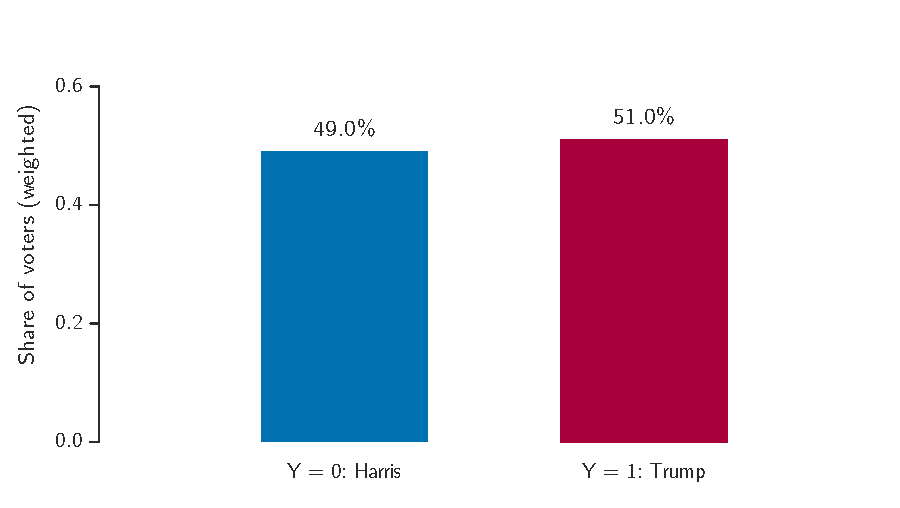
\includegraphics[height=0.76\textheight]{vote_marginal.pdf}
\end{figure}
\slidesource{Cooperative Election Study 2024: 42,028 respondents who reported voting for Trump or Harris; shares weighted by the survey weight}

}

\frame{
\frametitle{Vote and Education}

\vspace{-.2cm}
\begin{figure}[ht] \centering
        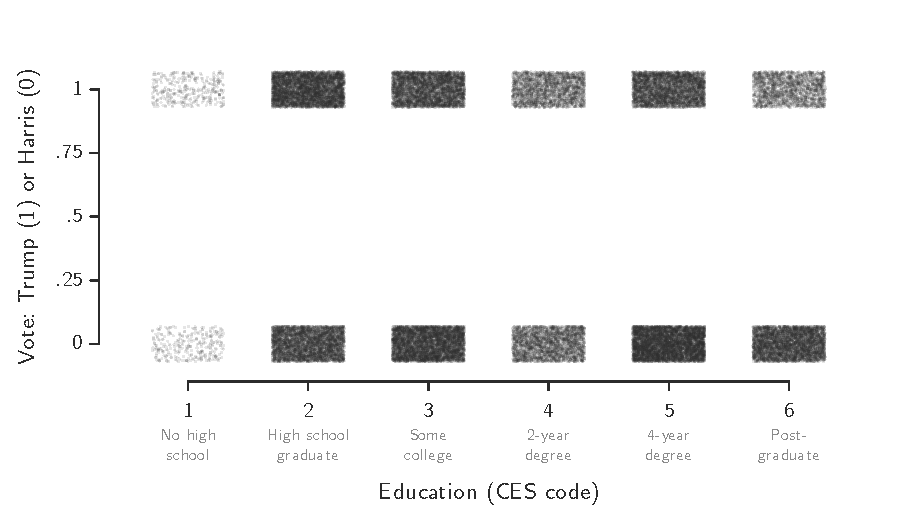
\includegraphics[height=0.76\textheight]{educ_vote_scatter.pdf}
\end{figure}
\slidesource{Cooperative Election Study 2024: 42,028 respondents who reported voting for Trump or Harris; shares weighted by the survey weight}

}

\frame{

\frametitle{Distribution of vote given education $p(y|x)$}

\vspace{-.2cm}
\begin{figure}[ht] \centering
        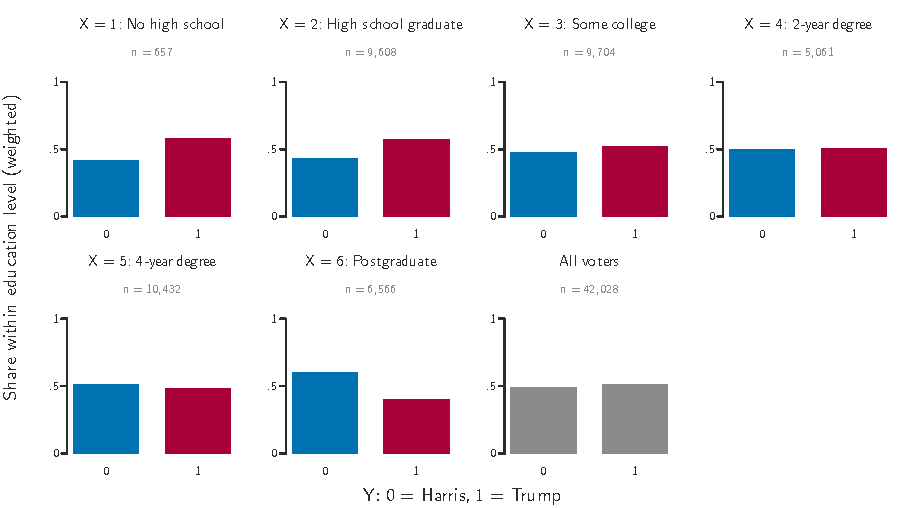
\includegraphics[height=0.76\textheight]{educ_vote_bars.pdf}
\end{figure}
\slidesource{Cooperative Election Study 2024: 42,028 respondents who reported voting for Trump or Harris; shares weighted by the survey weight}

}

\frame{
\frametitle{Nonparametric Regression with Discrete $X$}

\begin{itemize}
\item With a 0/1 outcome, each panel comes down to one number, the share voting Trump \bigskip
\item That share is the mean of $Y$, so it is the summary we want: $E[Y |X]$\bigskip
\item Here our $X$ variable education has a small number of levels (6) and many observations in each level (at least 657) \bigskip
\item In situations like this we can estimate $E[Y |X=x]$ as the sample mean of $Y$ at
each observed level $x$ of $X$\bigskip
\item We use a weighted mean: each respondent counts in proportion to the CES survey weight, which corrects for groups the survey reached too often or too rarely
\end{itemize}

}



\frame{
\frametitle{Nonparametric Regression with Discrete $X$}

\vspace{-.2cm}
\begin{figure}[ht] \centering
        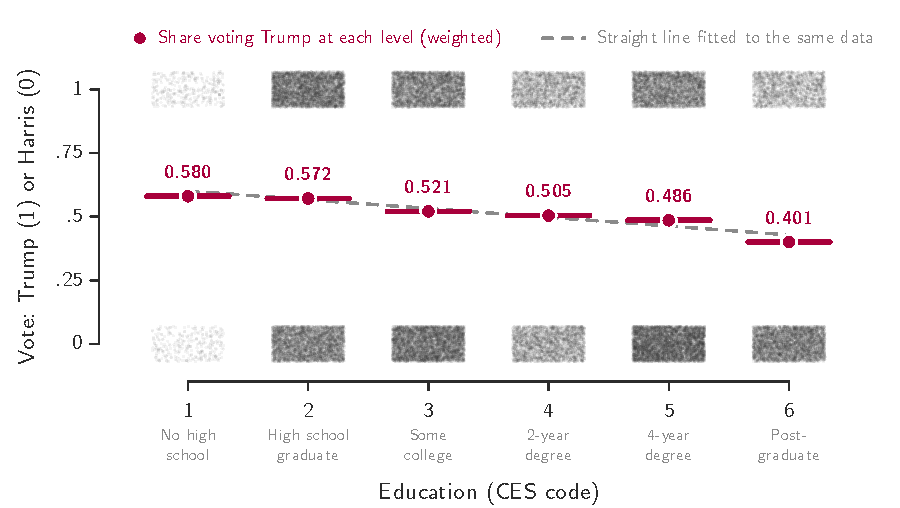
\includegraphics[height=0.76\textheight]{educ_vote_means.pdf}
\end{figure}
\slidesource{Cooperative Election Study 2024: 42,028 respondents who reported voting for Trump or Harris; shares weighted by the survey weight}

}

\frame{
\frametitle{Nonparametric Regression}

\begin{itemize}
\item The share voting Trump falls as education rises, but not along a straight line in the 1--6 code
  \begin{itemize}
  \item Flat between the two lowest levels: 58.0\% and 57.2\%
  \item A sharp drop at postgraduate degrees: 48.6\% to 40.1\%
  \item ``Some college'' and ``2-year degree'' are not obviously ordered, another reason not to force a line through a code
  \item No high school has the fewest respondents (657), so its share is the least precise
  \end{itemize}\medskip
\item Estimating $E[Y|X=x]$ level by level makes minimal assumptions
\item This method does not impose any specific \alert{functional form}
  on the relationship between $Y$ and $X$ (i.e. the shape of $E[Y|X]$)
\item $\rightarrow$ It is called a \alert{nonparametric
    regression}\medskip

\item It works well as long as
  \begin{itemize}
  \item $X$ is discrete
  \item there are a small number of values of $X$
  \item a small number of $X$ variables
  \item a lot of observations at each $X$ value
  \end{itemize}
\pause
\item But what do we do when $X$ is continuous and has many values?
\end{itemize}

}

\subsection{Continuous $X$}

\frame{
\frametitle{Nonparametric Regression with Continuous $X$}

Consider the 2024 presidential election in U.S. counties:\smallskip
\begin{itemize}
  \item 3,034 counties, from under 0.1 people per square mile (rural Texas) to about 72,000 (Manhattan)\bigskip
  \item We're interested in the relationship between:
  \begin{itemize}
    \item $Y$: Republican (Trump) share of the two-party vote, in \%
    \item $X$: log population density, the log of people per square mile \\
      ($X = 0$: 1 person; $X = 4.6$: 100 people; $X = 6.9$: 1,000 people)
  \end{itemize}\bigskip
  \item For the next slides we use a random sample of 200 counties, so each point can be seen; we come back to all 3,034 at the end
\end{itemize}
\slidesource{MIT Election Data and Science Lab; Census ACS 2019--23 and 2023 Gazetteer; N = 3,034 counties (Alaska, Connecticut, Louisiana and 7 other counties excluded)}

}


\frame{
\frametitle{Nonparametric Regression with Continuous $X$}
\vspace{-.2cm}
\begin{figure}[ht] \centering
        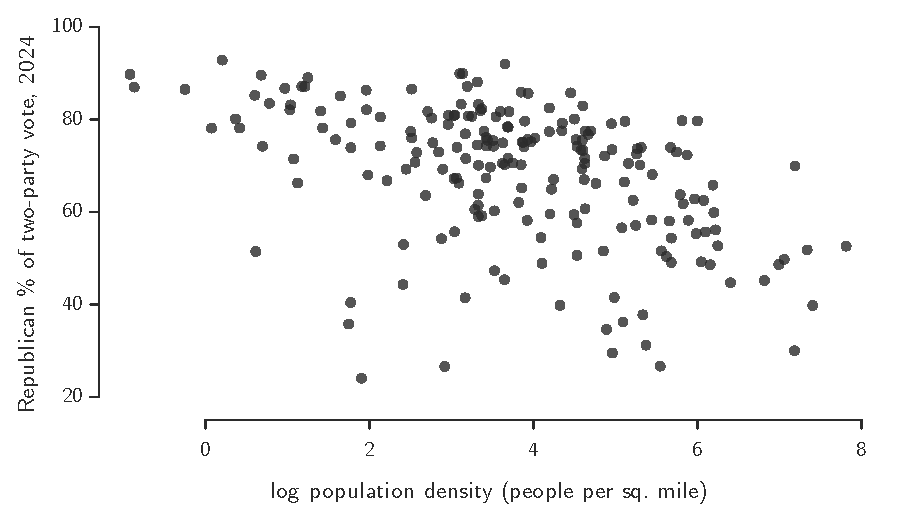
\includegraphics[height=0.75\textheight]{county_scatter.pdf}
\end{figure}
\slidesource{A random sample of 200 counties (seed 450) from the 3,034 above. MIT Election Data and Science Lab; Census ACS 2019--23 and 2023 Gazetteer}

}




\frame{
\frametitle{Uniform Kernel Regression: Simple Local Averages}
\small
\begin{itemize}
\item One approach is to use a \alert{moving local average} to
  estimate $E[Y |X]$
\item Calculate the average of the observed $y$ points that have $x$
  values in the interval $[x_0 - h \,,\, x_0 + h]$
\item $h = $ some positive number (called the \alert{bandwidth})
\pause
%\[
%\widehat E[Y|X=x_0]=\frac{\sum_{i \,\in\, [x_0 - h \,,\, x_0 + h]} Y_i}{\sum_{i \, \in \, [x_0 - h \,,\, x_0 + h]} 1}
%\]
%\item Can also do this by averaging the y values of the data points that are the
%k-nearest neighbors to x
%\item The approach is called a \alert{kernel regression} with a \alert{uniform or rectangular kernel} \bigskip
 %   \item In Stata:\texttt{ kdensity Y, kernel(rectangle)}
\item \alert{Uniform kernel}: every observation in the interval is
  equally weighted
\begin{figure}[ht] \centering
\begin{tikzpicture}[x=11mm, y=22mm, font=\scriptsize]
  \draw[->, gray] (-2.6,0) -- (2.6,0) node[right, CourseInk] {$u$};
  \draw[->, gray] (-2.6,0) -- (-2.6,0.95) node[above, CourseInk] {$K(u)$};
  \foreach \t in {-2,-1,0,1,2} \draw[gray] (\t,0) -- (\t,-0.04) node[below, CourseInk] {$\t$};
  \draw[gray] (-2.6,0) -- (-2.68,0) node[left, CourseInk] {$0$};
  \draw[gray] (-2.6,0.5) -- (-2.68,0.5) node[left, CourseInk] {$\tfrac12$};
  \draw[gray, densely dotted] (-2.6,0.5) -- (-1,0.5);
  \draw[very thick, Cardinal] (-2.5,0) -- (-1,0) -- (-1,0.5) -- (1,0.5) -- (1,0) -- (2.5,0);
\end{tikzpicture}
\end{figure}
\pause
\item This gives the \alert{uniform kernel regression}:
\[
\widehat E[Y|X=x_0]=\frac{\sum_{i=1}^N K((X_i-x_0)/h)
  Y_i}{\sum_{i=1}^N K((X_i-x_0)/h)}
 \ \text{where} \ K(u) = \frac12 \,\mathbf{1}_{\{|u|\leq1\}}
\]
\end{itemize}
% Gov 2000 credit removed 2026-10-11 (Yiqing): the figures (code/fig_kernel.R, code/fig_regression.R), data and example are ours.
}




\frame{\frametitle{Kernel Regression: Simple Local Averages}
\begin{figure}[ht] \centering
        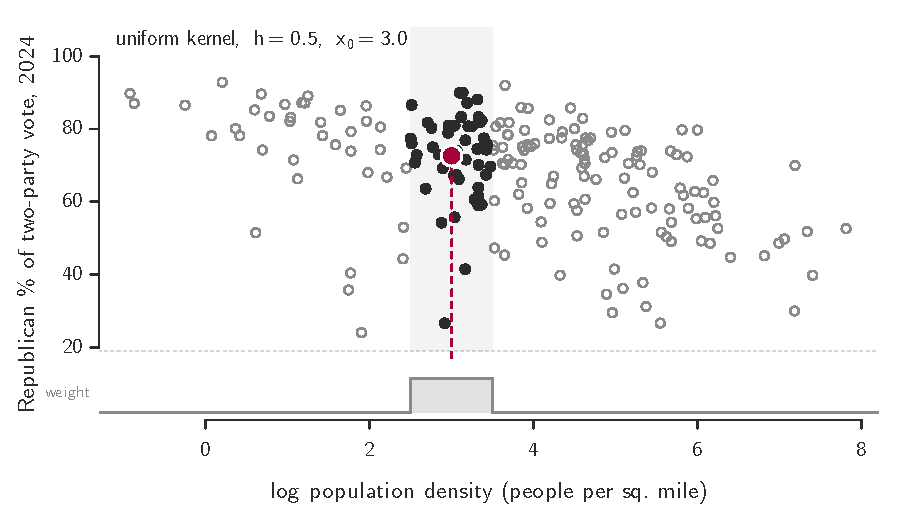
\includegraphics[height=0.81\textheight]{kernel_unif_1.pdf}
\end{figure}
}
\frame{\frametitle{Kernel Regression: Simple Local Averages}
\begin{figure}[ht] \centering
        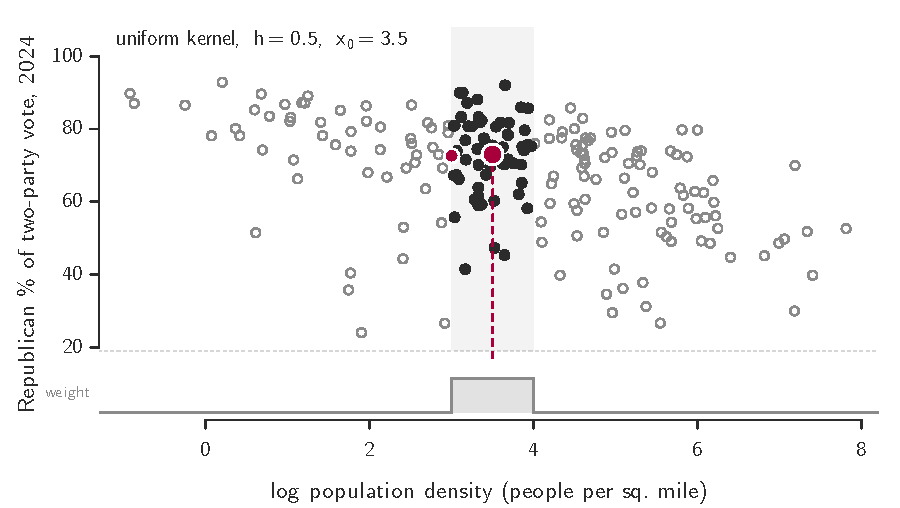
\includegraphics[height=0.81\textheight]{kernel_unif_2.pdf}
\end{figure}
}
\frame{\frametitle{Kernel Regression: Simple Local Averages}
\begin{figure}[ht] \centering
        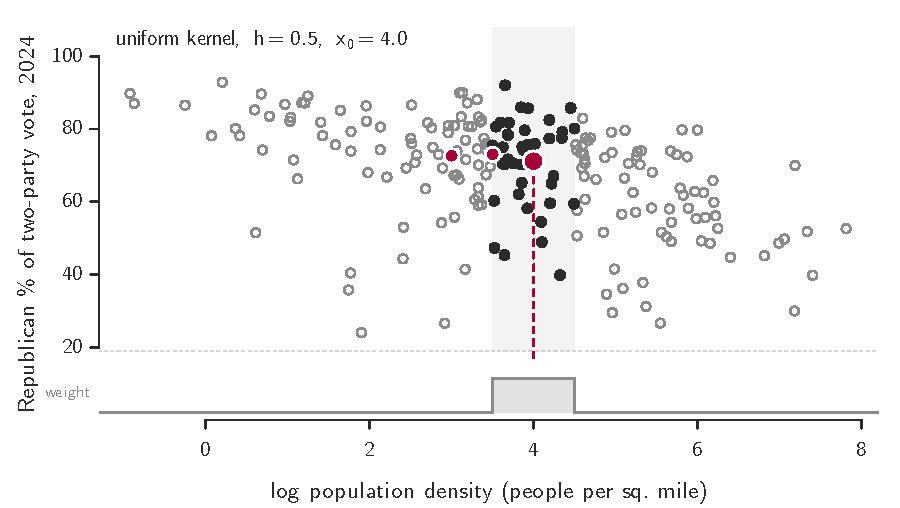
\includegraphics[height=0.81\textheight]{kernel_unif_3.pdf}
\end{figure}
}

\frame{\frametitle{Kernel Regression: Simple Local Averages}
\begin{figure}[ht] \centering
        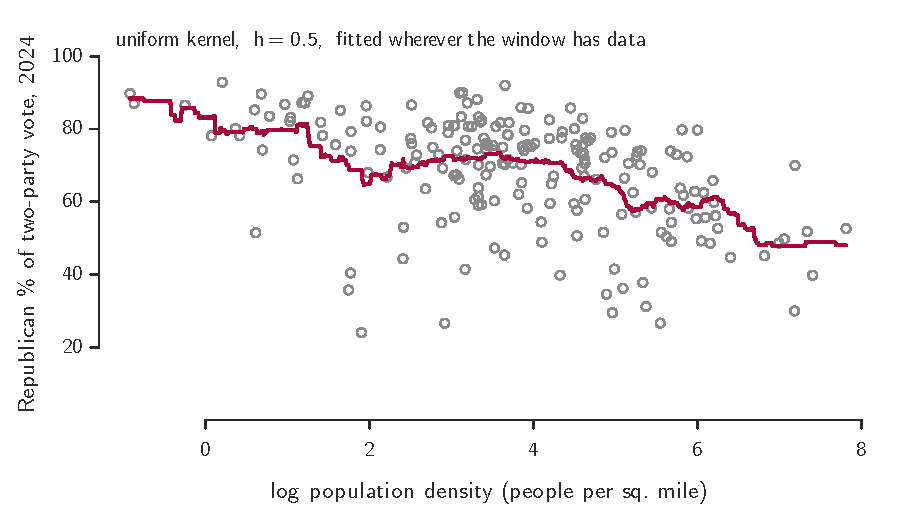
\includegraphics[height=0.81\textheight]{kernel_unif_4.pdf}
\end{figure}

}
\frame{
\frametitle{Changing the Bandwidth}

\begin{figure}[ht] \centering
        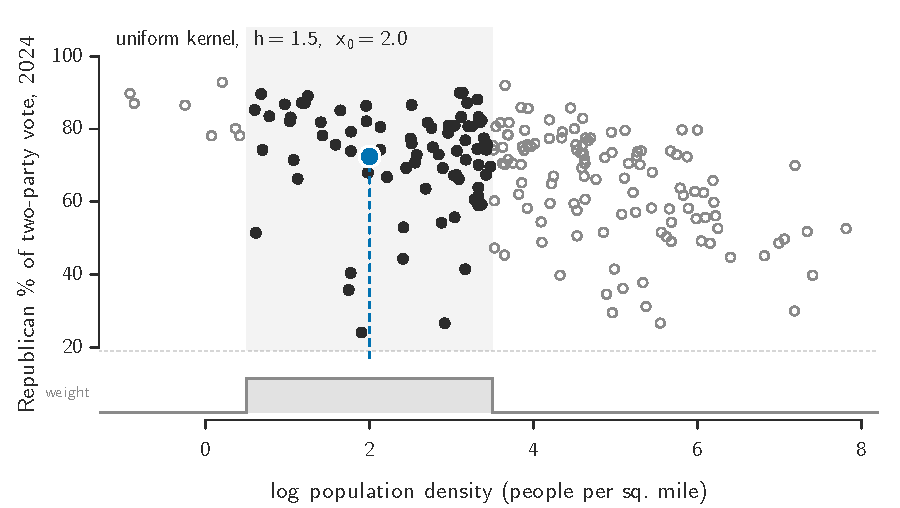
\includegraphics[height=0.81\textheight]{kernel_unif_wide_1.pdf}
\end{figure}

}

\frame{

\frametitle{Changing the Bandwidth}
\begin{figure}[ht] \centering
        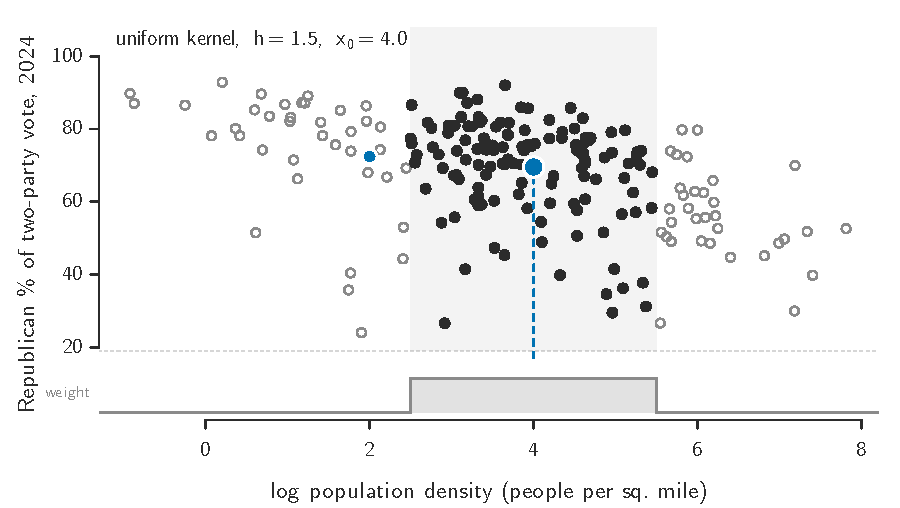
\includegraphics[height=0.81\textheight]{kernel_unif_wide_2.pdf}
\end{figure}

}

\frame{

\frametitle{Changing the Bandwidth}
\begin{figure}[ht] \centering
        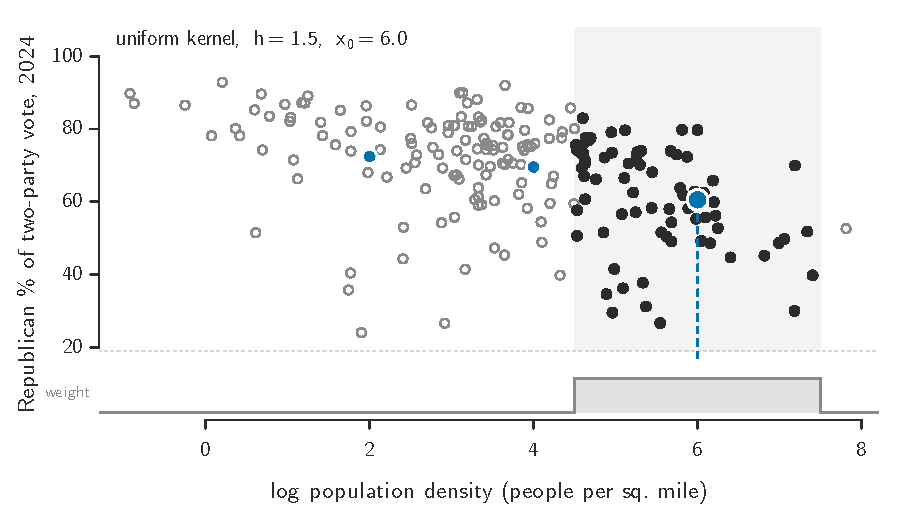
\includegraphics[height=0.81\textheight]{kernel_unif_wide_3.pdf}
\end{figure}

}

\frame{

\frametitle{Narrow and Wide Bandwidth}
\begin{figure}[ht] \centering
        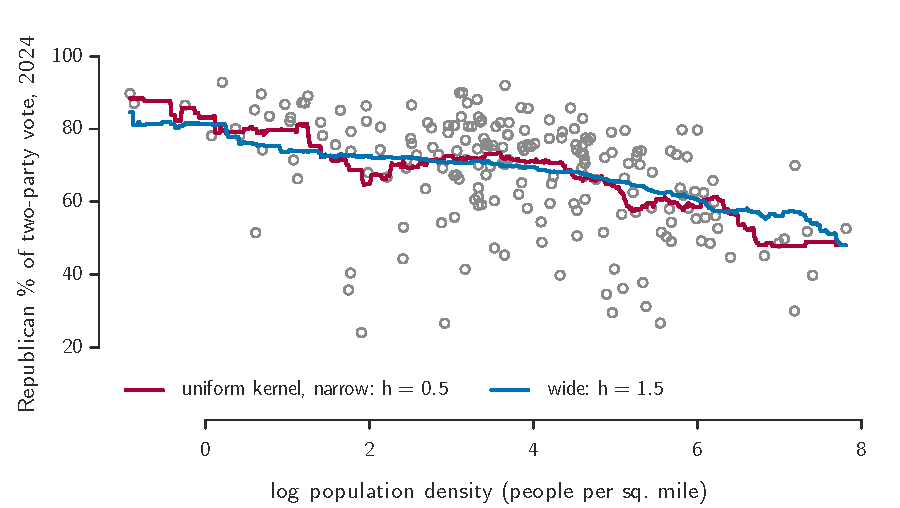
\includegraphics[height=0.81\textheight]{kernel_unif_both.pdf}
\end{figure}

}



\frame{
\frametitle{Kernel Regression: Weighted Local Averages}
\small
\begin{itemize}
  \item Another approach is to construct \alert{weighted local
      averages}
  \item Data points that are closer to $x_0$ get more weight than points farther away
\end{itemize}
\begin{enumerate}
  \item decide on a symmetric, non-negative \alert{kernel weight function} $K$
    that is zero outside $[-1,1]$ and falls as $|u|$ grows (e.g. Epanechnikov)
\begin{figure}[ht] \centering
\begin{tikzpicture}[x=11mm, y=22mm, font=\scriptsize]
  \draw[->, gray] (-2.6,0) -- (2.6,0) node[right, CourseInk] {$u$};
  \draw[->, gray] (-2.6,0) -- (-2.6,0.95) node[above, CourseInk] {$K(u)$};
  \foreach \t in {-2,-1,0,1,2} \draw[gray] (\t,0) -- (\t,-0.04) node[below, CourseInk] {$\t$};
  \draw[gray] (-2.6,0) -- (-2.68,0) node[left, CourseInk] {$0$};
  \draw[gray] (-2.6,0.75) -- (-2.68,0.75) node[left, CourseInk] {$\tfrac34$};
  \draw[gray, densely dotted] (-2.6,0.75) -- (0,0.75);
  \draw[very thick, Cardinal] (-2.5,0) -- (-1,0)
    -- plot[domain=-1:1, samples=41] (\x, {0.75*(1-(\x)*(\x))}) -- (2.5,0);
\end{tikzpicture}
\end{figure}
  \item compute weighted average of the observed $y$ points that
    have $x$ values in the bandwidth interval $[x_0 - h \,,\, x_0 + h]$ e.g.
\[
\widehat E[Y|X=x_0]=\frac{\sum_{i=1}^N K((X_i-x_0)/h) Y_i}{\sum_{i=1}^N K((X_i-x_0)/h)} \mbox{ where } K(u) = \frac{3}{4}(1-u^2) \,\mathbf{1}_{\{|u|\leq1\}}
\]
\end{enumerate}
%\item In Stata: \bigskip
%\item How will the weighted averaging affect our estimate of $E[Y|X=x]$ compared to the uniform kernel?

}


\frame{
\frametitle{A Weight Function}
\begin{figure}[ht] \centering
        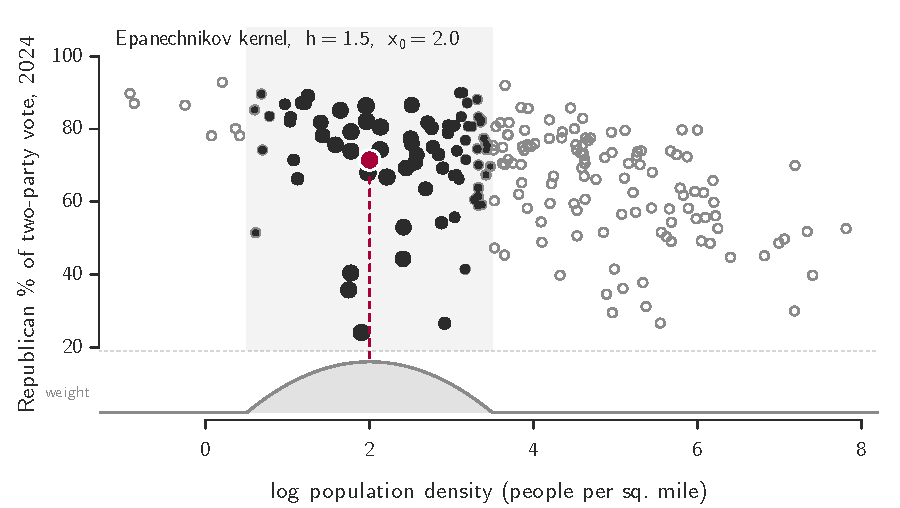
\includegraphics[height=0.81\textheight]{kernel_epa_1.pdf}
\end{figure}

}

\frame{
\frametitle{Weighted Local Averages}
\begin{figure}[ht] \centering
        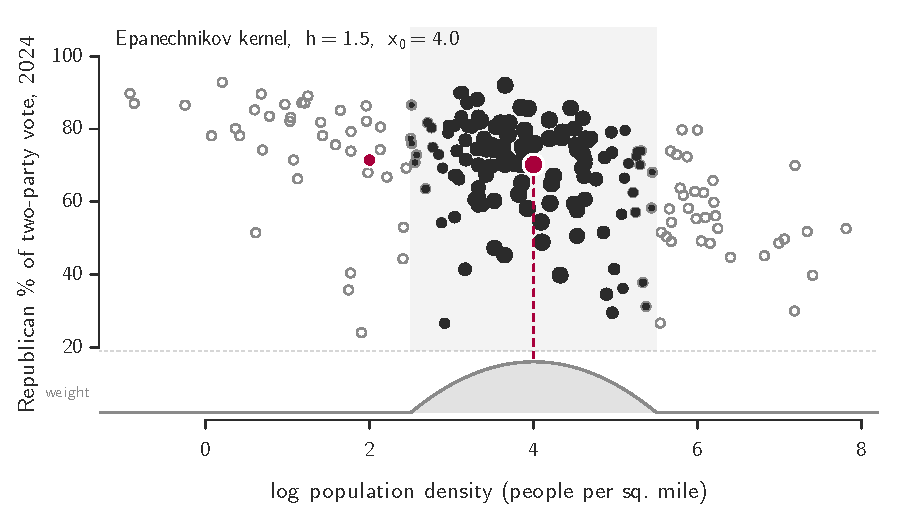
\includegraphics[height=0.81\textheight]{kernel_epa_2.pdf}
\end{figure}

}

\frame{
\frametitle{Weighted Local Averages}
\begin{figure}[ht] \centering
        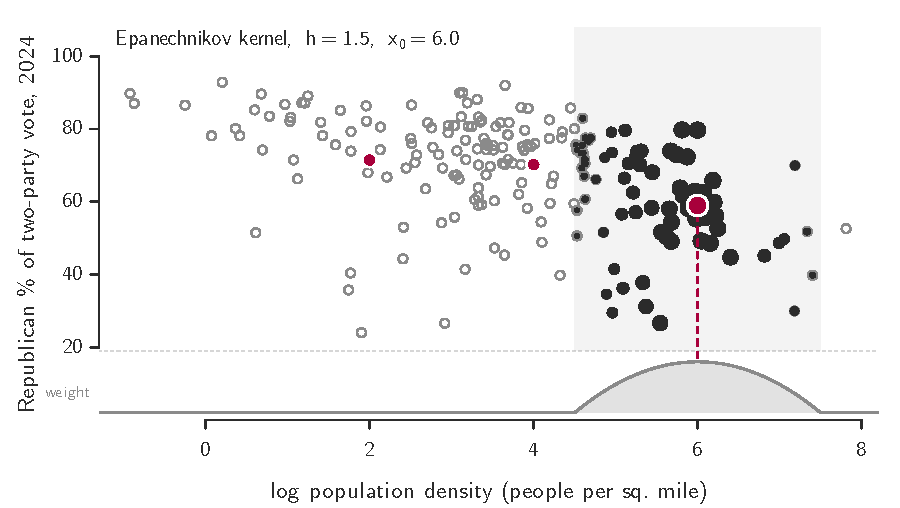
\includegraphics[height=0.81\textheight]{kernel_epa_3.pdf}
\end{figure}

}

\frame{
\frametitle{Kernel Regression: Weighted Local Averages}
\begin{figure}[ht] \centering
        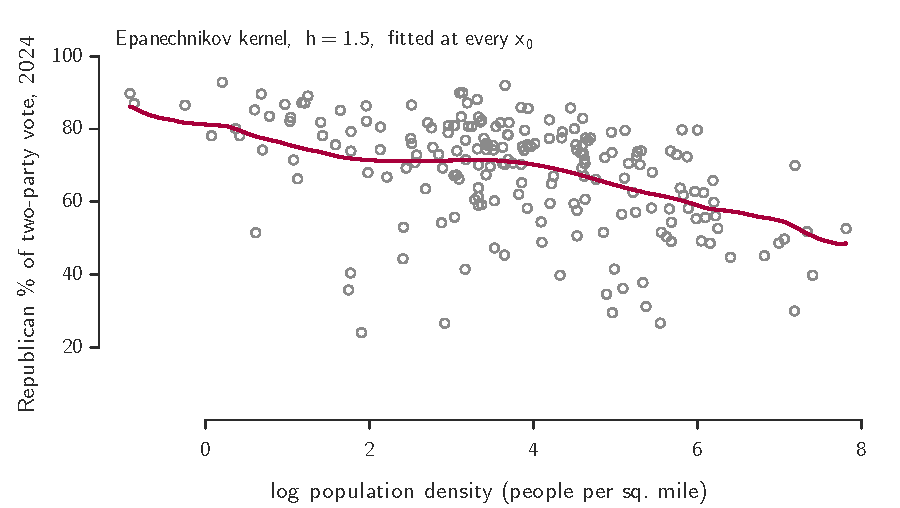
\includegraphics[height=0.81\textheight]{kernel_epa_4.pdf}
\end{figure}

}

\frame{
\frametitle{Changing the Bandwidth}
\begin{figure}[ht] \centering
        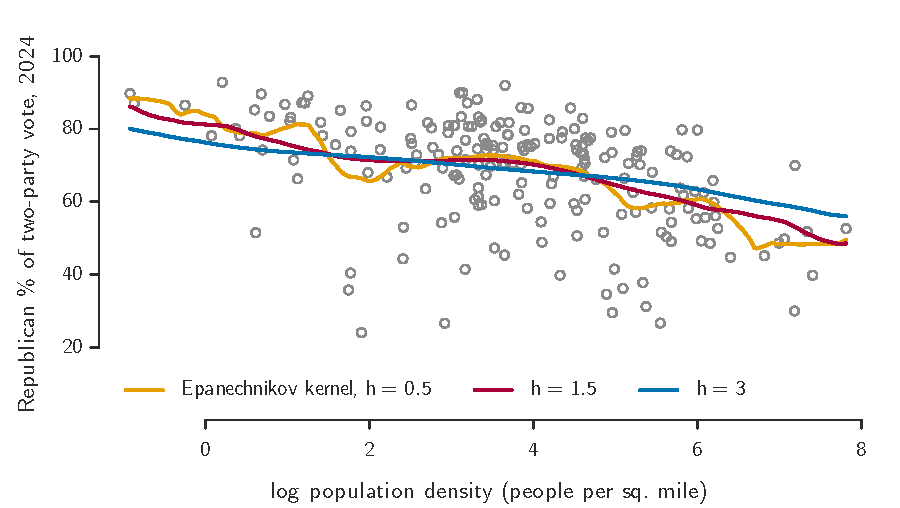
\includegraphics[height=0.81\textheight]{kernel_epa_bw.pdf}
\end{figure}

}

\subsection{Bias-Variance Tradeoff}

\frame{
\frametitle{Bias-Variance Tradeoff}

\begin{itemize}
\item When choosing an estimator $\widehat{E}[Y|X]$ for $E[Y|X]$, we face a \alert{bias-variance tradeoff}\bigskip
\item Notice that we can choose models with various levels of flexibility:
\begin{itemize}
  \item A very \alert{flexible estimator} allows the shape of the function to vary \\ (e.g. a kernel regression with a small bandwidth)\bigskip
  \item A very \alert{inflexible estimator} restricts the shape of the function to a particular form \\
    (e.g. a kernel regression with a very wide bandwidth)\bigskip
\end{itemize}
\end{itemize}

%\item We can chose a very flexible model  that allows us to approximate
%
%
%\item $E[Y|x]$ is the parameter(s) of interest (the conditional mean or expectation for a given value of $x$)
%\item  is the estimator of the parameter of interest.
%\item The estimates are the red lines (the constant functions).
%\item Since the previous plot involves actual data, we can't know the true value of the parameter, or say much about the behavior of the estimator.
%\end{itemize}
}


\frame{
\frametitle{Hypothetical True Distribution}
\begin{itemize}
  \item Let's conduct a simulation experiment to actually see the tradeoff
  \item Suppose we have the following population distribution:
\vspace{-.1in}
\end{itemize}
\begin{figure}[ht] \centering
        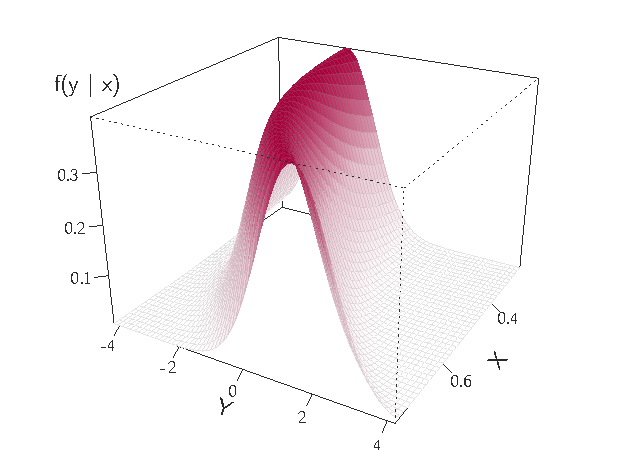
\includegraphics[height=0.67\textheight]{bv_true_persp.pdf}
\end{figure}
}

\frame{
\frametitle{Hypothetical True Distribution}
\begin{itemize}
  \item Another way of representing the same population distribution:
\vspace{-.2em}
\begin{figure}[ht] \centering
        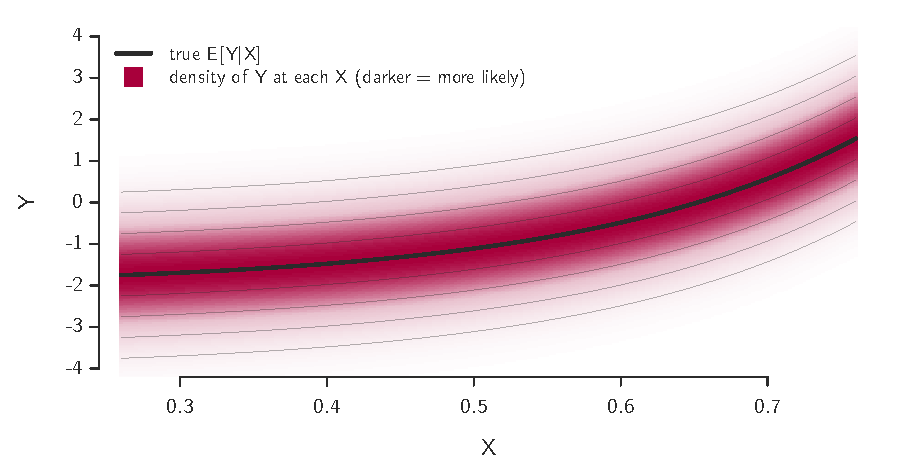
\includegraphics[height=0.62\textheight]{bv_true_contour.pdf}
\end{figure}
 \item From this distribution we draw 2,000 simulated data sets: $X$ is held at 32 evenly spaced values from 0.26 to 0.76, and each $Y$ is drawn from $f(y|x)$.
\end{itemize}
}

%\frame{
%\frametitle{Simulating Conditional Data}
%
%
%\begin{enumerate}
%\item Start with the $x$ values in the data.
%\item Use the conditional distribution $f(y|x)$ to simulate a $y$ value for each $x$ value.
%\item Repeat for as many simulated data sets as necessary.
%\end{enumerate}
%
%
%}

\frame{
\frametitle{An Example of a Simulated Data Set}
\begin{figure}[ht] \centering
        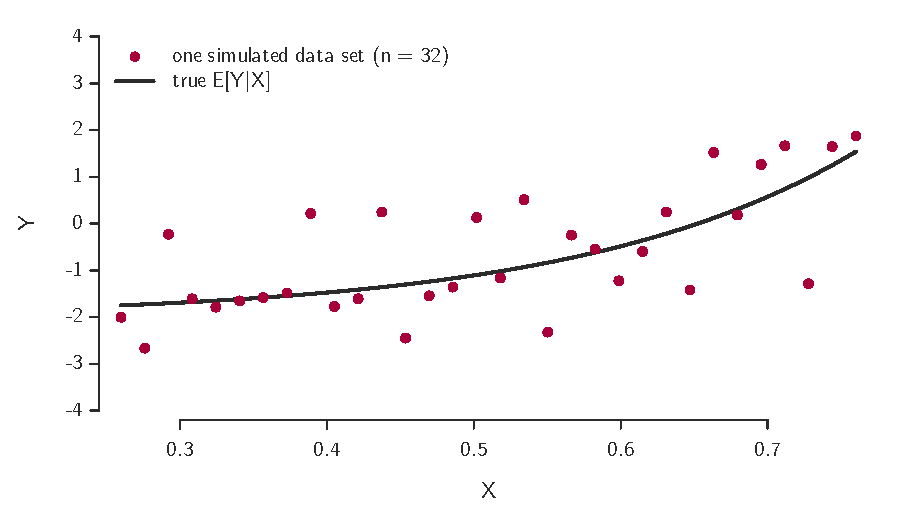
\includegraphics[height=0.81\textheight]{bv_sim_data.pdf}
\end{figure}
}


\frame{
\frametitle{Two Estimators}
\small
\begin{itemize}
  \item For each simulated data set, we apply two simple estimators of $E[Y|X]$:
    \begin{itemize}
      \item Divide $X$ into {\bf 4} ranges and take the mean for each
      \item Divide $X$ into {\bf 8} ranges and take the mean for each
    \end{itemize}
  \item We then evaluate how well these estimators do in terms of bias and variance.
\end{itemize}
\vspace{-.2in}
\begin{figure}[ht] \centering
        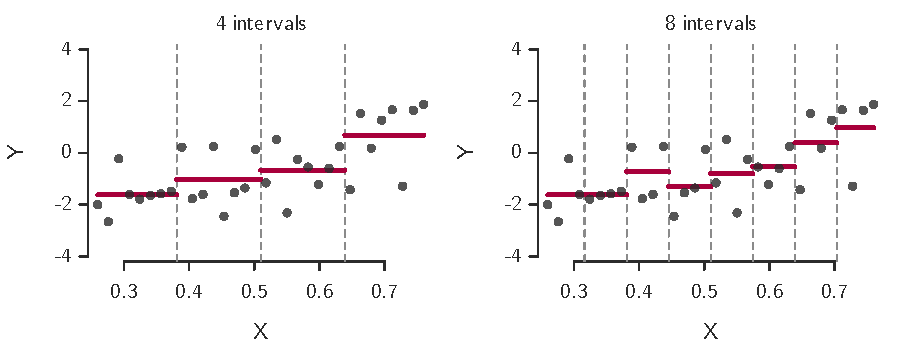
\includegraphics[height=0.58\textheight]{bv_two_estimators.pdf}
\end{figure}
}


\frame{
\frametitle{Simulated Distribution of Estimates: 4 Intervals}
\begin{figure}[ht] \centering
        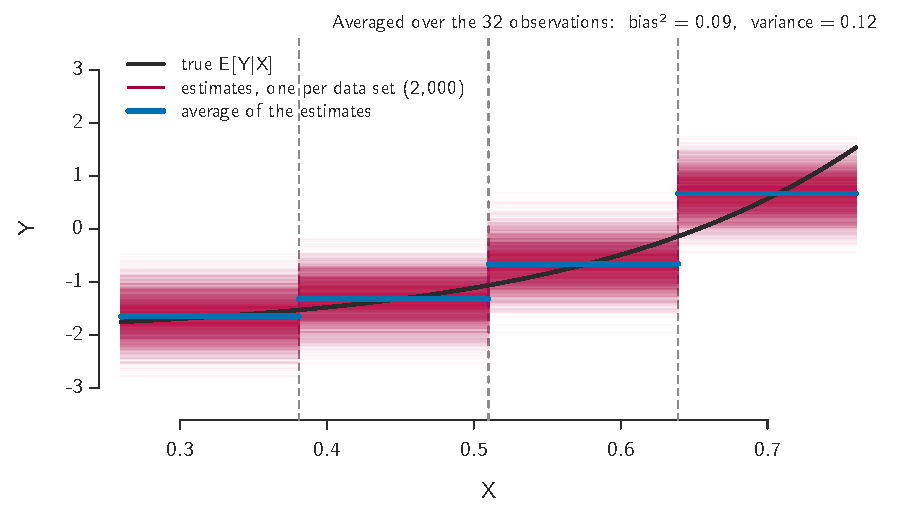
\includegraphics[height=0.81\textheight]{bv_bias_4bins.pdf}
\end{figure}

}

\frame{
\frametitle{Simulated Distribution of Estimates: 8 Intervals}
\begin{figure}[ht] \centering
        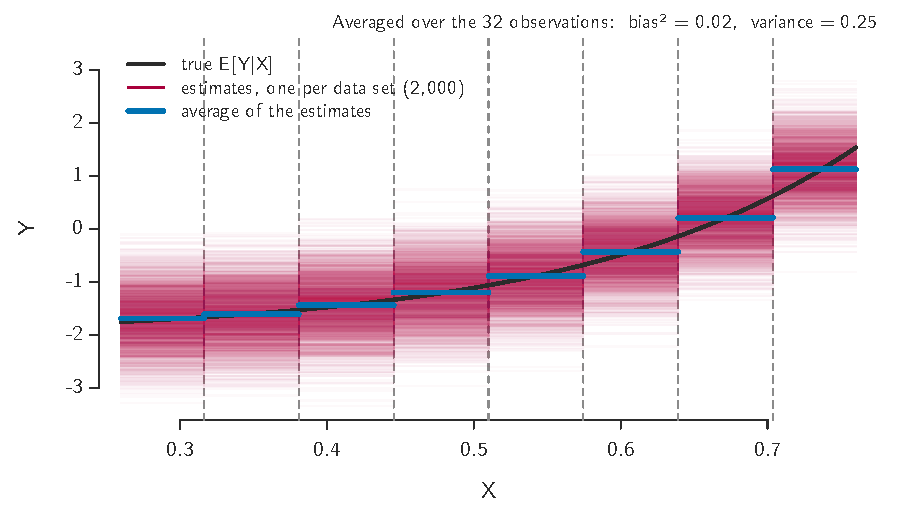
\includegraphics[height=0.81\textheight]{bv_var_8bins.pdf}
\end{figure}

}

\frame{
\frametitle{Bias-Variance Tradeoff}

\begin{itemize}
\item In this comparison, the less ``flexible'' estimator (4 ranges) has more bias\bigskip
\item and the more ``flexible'' estimator (8 ranges) has more variance\bigskip
\item So choosing the flexibility means balancing bias against variance\bigskip
\item With more data (or fewer variables) we can ``afford'' a more flexible estimator, and both can shrink
\end{itemize}

}

\section{Linear Regression}

\frame{
\frametitle{Parametric Approach: Linear Regression}
\begin{itemize}
  \item Linear regression works by assuming a linear parametric form for
  the conditional expectation function:
$$
E[Y|X] = \beta_0 + X\,\beta_1
$$
\item Conditional expectation defined by only two \alert{coefficients} which are estimated from the data:
\begin{itemize}
  \item $\beta_0$ is called the \alert{intercept} or \alert{constant}
  \item $\beta_1$ is called the \alert{slope coefficient}
\end{itemize}\bigskip
\item Notice that the linear functional form imposes a constant slope
\item Assumption: Change in $E[Y|X]$ is the same at all values of $X$
\bigskip
\item Geometrically, the linear regression function will look like: \smallskip
\begin{itemize}
  \item A \alert{line} in cases with a single $X$ variable\smallskip
  \item A \alert{plane} in cases with two $X$ variables\smallskip
  \item A \alert{hyperplane} in cases with more than two $X$ variables\bigskip
\end{itemize}
\end{itemize}

}

\begin{frame}[fragile]
\frametitle{Parametric Approach: Linear Regression in R}
\footnotesize
\begin{Verbatim}[frame=single, label=R Code, commandchars=\\\{\}]
> counties <- read.csv("county_pres.csv")
> counties$rep24 <- 100 * counties$rep2p_2024   # Republican % of two-party vote
> counties <- subset(counties, !is.na(rep24))    # counties with 2024 returns
> head(counties[, c("county", "state", "rep24", "pct_ba", "log_density")])
          county state   rep24  pct_ba log_density
1 Autauga County    AL 73.3589 28.2827    4.602467
2 Baldwin County    AL 79.3476 32.7976    5.016762
3 Barbour County    AL 57.4150 11.4647    3.331267
4    Bibb County    AL 82.3849 11.4682    3.571988
5  Blount County    AL 90.7769 15.5790    4.521148
6 Bullock County    AL 26.9589  8.9997    2.791669
\end{Verbatim}
\texttt{pct\_ba}: \% of adults 25 and older with a BA or higher. We now regress the Republican share on \texttt{pct\_ba}.
\slidesource{MIT Election Data and Science Lab; Census ACS 2019--23; N = 3,034 counties (Alaska, Connecticut, Louisiana and 7 other counties excluded)}

\end{frame}

\begin{frame}[fragile]
\frametitle{Parametric Approach: Linear Regression in R}
\scriptsize
\begin{Verbatim}[frame=single, label=R Code, commandchars=\\\{\}]
> lm.out <- lm(rep24 ~ pct_ba, data = counties)
> summary(lm.out)

Call:
lm(formula = rep24 ~ pct_ba, data = counties)

Residuals:
    Min      1Q  Median      3Q     Max
-66.800  -6.879   1.956   8.586  40.102

Coefficients:
            Estimate Std. Error t value Pr(>|t|)
(Intercept) \alert{89.00934}    0.61309  145.18   <2e-16 ***
pct_ba      \alert{-0.87431}    0.02342  -37.33   <2e-16 ***
---
Signif. codes:  0 `***' 0.001 `**' 0.01 `*' 0.05 `.' 0.1 ` ' 1

Residual standard error: 13.12 on 3032 degrees of freedom
Multiple R-squared:  0.3149,	Adjusted R-squared:  0.3147
F-statistic:  1393 on 1 and 3032 DF,  p-value: < 2.2e-16

\end{Verbatim}

\end{frame}



\frame{
\frametitle{Parametric Approach: Linear Regression}
\vspace{-.2cm}
\begin{figure}[ht] \centering
        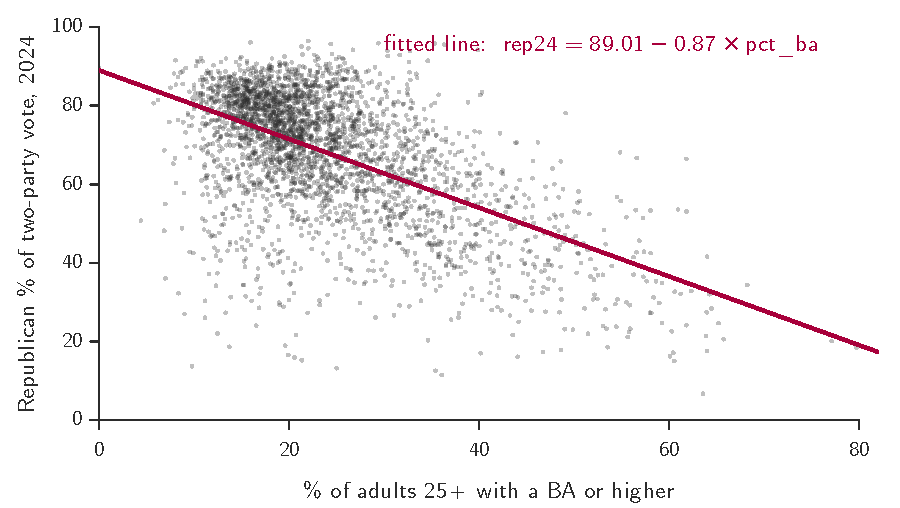
\includegraphics[height=0.75\textheight]{county_ols.pdf}
\end{figure}
\slidesource{MIT Election Data and Science Lab; Census ACS 2019--23; N = 3,034 counties (Alaska, Connecticut, Louisiana and 7 other counties excluded)}

}

%\frame{
%
%\frametitle{Linear Regression: Interpretation}
%Suppose we have computed coefficient estimates for our regression:
%$$
%Y = \hat{\beta}_0 + \hat{\beta}_1 X
%$$
%$$
%\widehat{\mbox{rep24}} = 89.0 - 0.87\,\mbox{pct\_ba}
%$$
%
%}

\frame[t]{
\frametitle{Linear Regression: Interpretation}
Suppose we have computed coefficient estimates for our regression:
$$
\widehat{Y} = \hat{\beta}_0 + \hat{\beta}_1 X
$$
$$
\widehat{\mbox{rep24}} = 89.0 - 0.87 \,\mbox{pct\_ba}
$$
\bigskip
\begin{overprint}
\onslide<2|handout:0>
Q: What does $\hat{\beta}_0$ tell us? \bigskip
\onslide<3|handout:1>
Q: What does $\hat{\beta}_0$ tell us? \bigskip

Substituting $0$ in for $x$ we see that $E[Y|X=0] = \beta_0$, so $\hat\beta_0$ estimates the average of $Y$ where $X=0$.\\ \bigskip

Our estimate of the average Republican share is 89.0\% for a county where no adult has a BA. Only one county is at 0\%: Loving County, TX, population 54. The next lowest is at 4.4\%. So this is an extrapolation beyond nearly all of the data.
\end{overprint}

}


\frame[t]{
\frametitle{Linear Regression: Interpretation}
Suppose we have computed coefficient estimates for our regression:
$$
\widehat{Y} = \hat{\beta}_0 + \hat{\beta}_1 X
$$
$$
\widehat{\mbox{rep24}} = 89.0 - 0.87 \,\mbox{pct\_ba}
$$
\bigskip
\begin{overprint}
\onslide<1|handout:0>
Q: What does $\hat{\beta}_1$ tell us?

\onslide<2|handout:1>
Q: What does $\hat{\beta}_1$ tell us? \bigskip

\alert{Sign}: The sign of the slope estimate $\hat\beta_1$ tells us if the fitted $\widehat{E}[Y|X]$
    increases or decreases with a change in $X$\\\medskip
    $\hat\beta_1>0$: $\widehat{E}[Y|X]$ increases with $X$\\\smallskip
    $\hat\beta_1<0$: $\widehat{E}[Y|X]$ decreases with $X$\\\smallskip
    $\hat\beta_1=0$: $\widehat{E}[Y|X]$ is flat in $X$
\end{overprint}

}

\frame[t]{
\frametitle{Linear Regression: Interpretation}
Suppose we have computed coefficient estimates for our regression:
$$
\widehat{Y} = \hat{\beta}_0 + \hat{\beta}_1 X
$$
$$
\widehat{\mbox{rep24}} = 89.0 - 0.87 \,\mbox{pct\_ba}
$$
\bigskip
\begin{overprint}
\onslide<1|handout:1>
Q: What does $\hat{\beta}_1$ tell us?

\bigskip

\alert{Magnitude}: The slope estimate $\hat\beta_1$ tells us \alert{how fast} $\widehat{E}[Y|X]$
    increases or decreases with a one unit change in $X$ \\

A one unit increase in $X$ is associated with a $\hat\beta_1$ unit increase in the fitted average of $Y$, $\widehat{E}[Y|X]$. \\

Here a county with 1 point more of its adults holding a BA has a fitted Republican share 0.87 points lower. A county with 10 points more has a share 8.7 points lower. These are observational data, so the slope describes a difference between counties. It is not an effect of education.
\end{overprint}
}


\frame{
\frametitle{Linear Regression: Justification}
\begin{itemize}
  \item Linear regression imposes a {\bf strong} assumption on $E[Y|X]$
  \item Why would we ever want to do this?\bigskip
\pause
  \begin{itemize}
    \item Theoretical reason to assume linearity \bigskip
    \item Ease of interpretation\bigskip
    \item Bias-variance tradeoff \bigskip
    \item Analytical derivation of sampling distributions (next few weeks) \bigskip
    \item We can make the model more flexible, even in a linear framework (e.g. we can add polynomials, use log transformations, etc.)
  \end{itemize}
\end{itemize}


}

\section{Combining Linear Regression with Nonparametric Regression}
\frame{
\frametitle{LOWESS}
\begin{itemize}
\item The moving local average methods for nonparametric regression
  didn't take into account how $y$ was
  \emph{changing} with $x$
\item We can incorporate this information by fitting a linear regression
within each band
\bigskip
\item Locally weighted scatterplot smoothing (\alert{LOWESS} or \alert{LOESS}):
\begin{enumerate}
  \item Pick a subset of the data that falls in the interval $[x_0 - h \,,\, x_0 + h]$
\smallskip
  \item Fit a line to this subset of the data ($=$ \alert{locally linear regression}),
    weighting the points by their distance to $x_0$ using a kernel function
\smallskip
  \item Use the fitted regression line to predict the expected value of $E[Y|X=x_0]$
  \end{enumerate}\bigskip
%For each $X=x_0$, minimize:
%\[
%\sum_{i=1}^N K((X_i-x_0)/h)(Y_i-b_0 - b_1 (X_i-x_0)^2.
%\]
%\item In Stata: \texttt{lowess Y X}
\item R's \texttt{loess()} sets the neighborhood by the nearest fraction \texttt{span} of the data (default 0.75), with tricube weights
\item In \texttt{R}, \texttt{loess(Y $\sim$ X, degree = 1)} fits local lines; the default, \texttt{loess(Y $\sim$ X)}, fits local quadratics

\end{itemize}

% requires a lot of data and computationally intense

}

%\frame{
%\frametitle{Local Linear Regression}
%\vspace{.3cm}
%\begin{figure}[ht] \centering
%        \scalebox{1}{\includegraphics{linBinChirot.pdf}}
%\end{figure}
%
%}

\frame{
\frametitle{Weighted Local Linear Regressions}
\begin{figure}[ht] \centering
        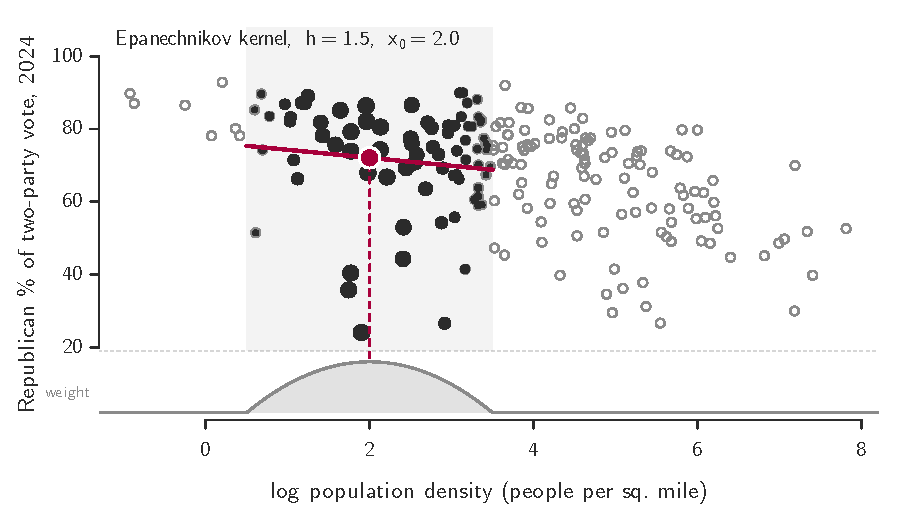
\includegraphics[height=0.81\textheight]{loclin_1.pdf}
\end{figure}

}

\frame{
\frametitle{Weighted Local Linear Regressions}
\begin{figure}[ht] \centering
        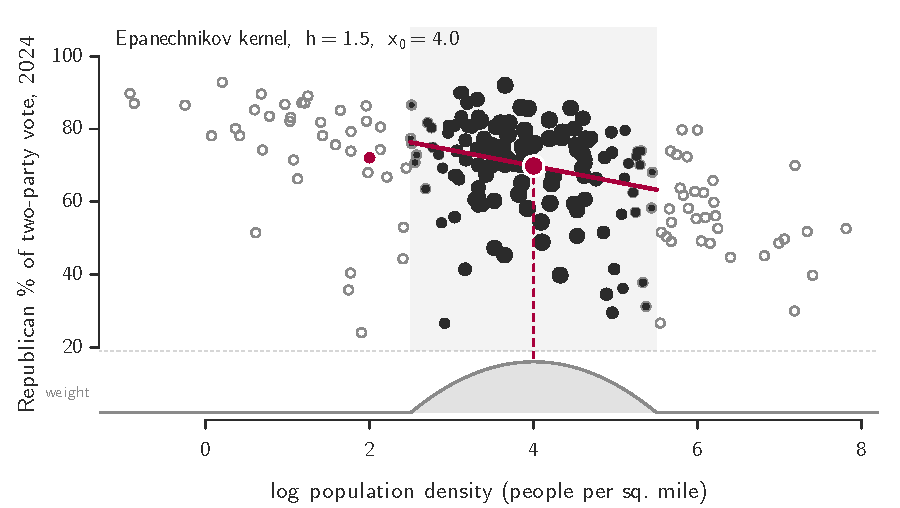
\includegraphics[height=0.81\textheight]{loclin_2.pdf}
\end{figure}

}

\frame{
\frametitle{Weighted Local Linear Regressions}
\begin{figure}[ht] \centering
        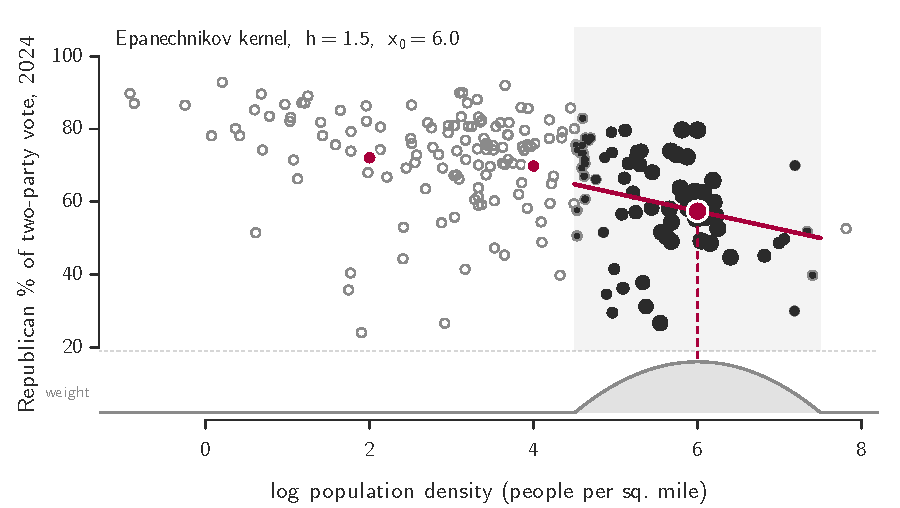
\includegraphics[height=0.81\textheight]{loclin_3.pdf}
\end{figure}

}

\begin{frame}[fragile]
\frametitle{LOESS Characterization of $E[Y|X]$}\vspace{.3cm}
\begin{Verbatim}[frame=single, label=R Code, commandchars=\\\{\}]
set.seed(450)
cty200 <- counties[sample(nrow(counties), 200), ]   # a random sample of 200
cty200 <- cty200[order(cty200$log_density), ]
lo.out <- loess(rep24 ~ log_density, data = cty200)
plot(rep24 ~ log_density, data = cty200)
lines(lo.out$fitted, x = lo.out$x, col = "red")
\end{Verbatim}
\end{frame}



\frame{
\frametitle{LOESS Characterization of $E[Y|X]$}
\begin{figure}[ht] \centering
        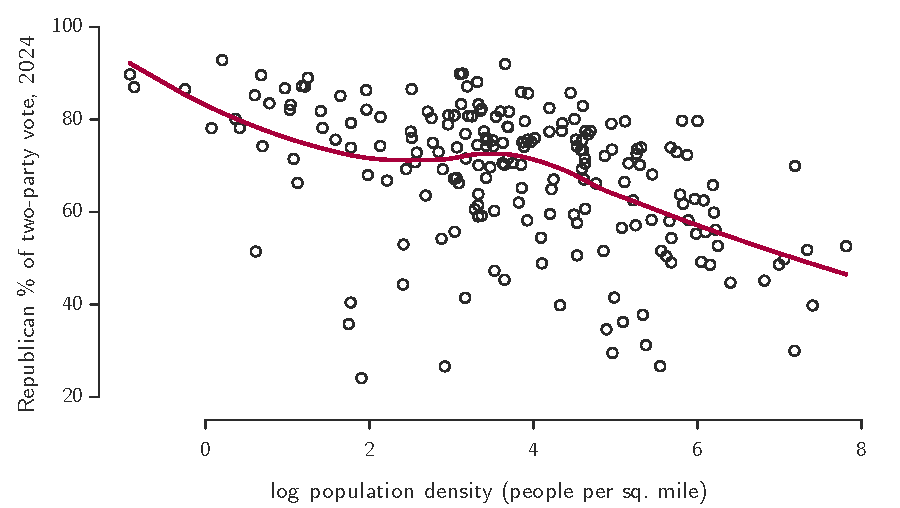
\includegraphics[height=0.81\textheight]{county_loess_base.pdf}
\end{figure}

}

\begin{frame}[fragile]
\frametitle{LOESS Characterization of $E[Y|X]$}\vspace{.3cm}
\begin{Verbatim}[frame=single, label=R Code, commandchars=\\\{\}]
library(ggplot2)

ggplot(cty200, aes(x = log_density, y = rep24)) +
  geom_point() +
  geom_smooth(method = "loess")
\end{Verbatim}
\end{frame}

\frame{
\frametitle{LOESS Characterization of $E[Y|X]$}
\begin{figure}[ht] \centering
        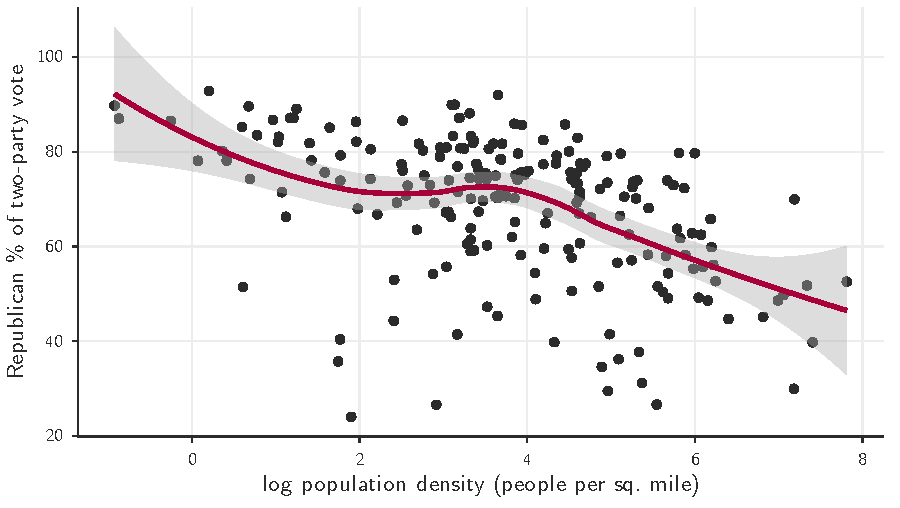
\includegraphics[height=0.81\textheight]{county_loess_gg.pdf}
\end{figure}

}

\begin{frame}[fragile]
\frametitle{LOESS Characterization of $E[Y|X]$}\vspace{.3cm}
\begin{Verbatim}[frame=single, label=R Code, commandchars=\\\{\}]
ggplot(cty200, aes(x = log_density, y = rep24)) +
  geom_point() +
  geom_smooth(method = "loess", span = 0.25, se = FALSE, aes(colour = "0.25")) +
  geom_smooth(method = "loess", span = 0.75, se = FALSE, aes(colour = "0.75")) +
  geom_smooth(method = "loess", span = 1,    se = FALSE, aes(colour = "1")) +
  labs(colour = "span")
\end{Verbatim}
\end{frame}

\frame{
\frametitle{LOESS Characterization of $E[Y|X]$}
\begin{figure}[ht] \centering
        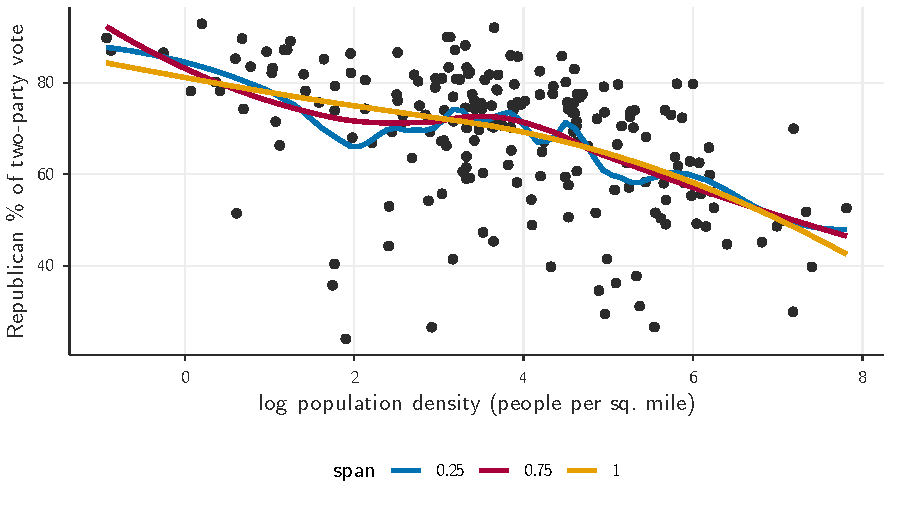
\includegraphics[height=0.81\textheight]{county_loess_spans.pdf}
\end{figure}

}

\begin{frame}[fragile]
\frametitle{GAM Characterization of $E[Y|X]$}\vspace{.3cm}
\begin{Verbatim}[frame=single, label=R Code, commandchars=\\\{\}]
ggplot(counties, aes(x = log_density, y = rep24)) +
  geom_point(size = 0.5, alpha = 0.2) +
  geom_smooth(method = "gam", formula = y ~ s(x, bs = "cs"))
\end{Verbatim}
\medskip
\texttt{s(x)} is a smooth function of $x$. A GAM chooses how wiggly it is from the data. Now we use all 3,034 counties. The GAM picks a curve with 5.9 effective degrees of freedom (a straight line has 1). The curve falls about 3 points per unit of log density up to 4.5 (90 people per square mile), then about 9.\medskip

With many more data points, the bandwidth choice matters less. With all 3,034 counties, LOESS curves with span 0.25 and span 0.75 differ by at most 2.2 points. In the sample of 200 they differ by up to 5.7 points (both over the middle 96\% of densities).
\end{frame}

\frame{
\frametitle{GAM Characterization of $E[Y|X]$}
\vspace{-.2cm}
\begin{figure}[ht] \centering
        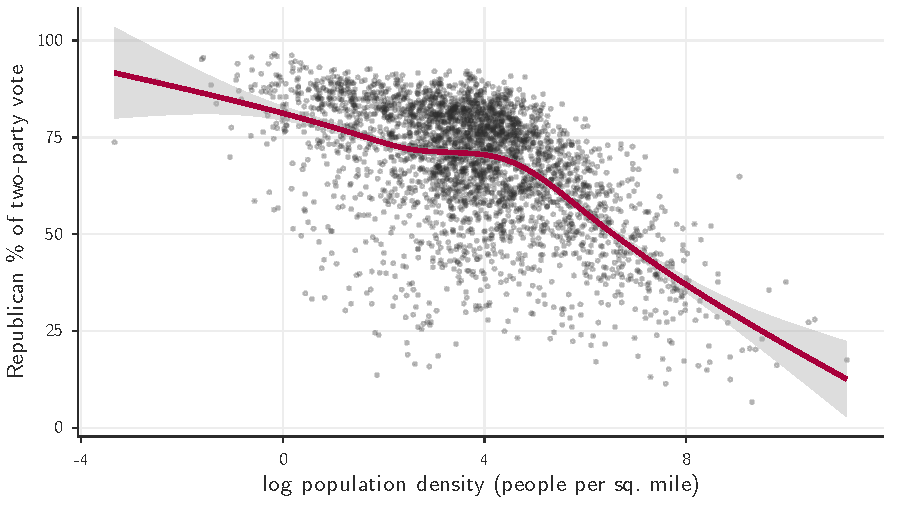
\includegraphics[height=0.70\textheight]{county_gam.pdf}
\end{figure}
\slidesource{MIT Election Data and Science Lab; Census ACS 2019--23 and 2023 Gazetteer; N = 3,034 counties (Alaska, Connecticut, Louisiana and 7 other counties excluded)}

}

%\begin{frame}
%  \frametitle{Required readings}
%Due Wednesday next week:
%\begin{itemize}
%\item Wooldrige: Chapter 2\\\bigskip
%\item Acock: Ch 5 + 6 (if you lack Stata background)
%\end{itemize}

%\section{Interpreting Regression}
%
%\frame{
%\frametitle{Regression as a Predictive Model}
%\begin{itemize}
%  \item Regression can also be used to \alert{predict} new observations\medskip
%  \item e.g. linear regression:
%  \begin{itemize}
%    \item Find estimates $\widehat{\beta}_0, \widehat{\beta}_1$ of
%    $\beta_0, \beta_1$ based on the \emph{in-sample data}
%    \item To find the expected value of $Y$ for an \emph{out-of-sample} data
%    point with $X=x_{new}$, calculate:
%$$
%\widehat{E}[Y|X=x_{new}] = \widehat{\beta}_0 + \widehat{\beta}_1 x_{new}
%$$
%  \end{itemize}
%  \item You can use the same procedure to estimate the \alert{expected difference}:
%$$ \widehat{E}[y|X=x_{new,1}] - \widehat{E}[y\mid X=x_{new,2}] \ = \
%    \widehat{\beta}_1(x_{new,1} - x_{new,2}) $$
%
% \item In a predictive model, $\beta_1$ is interpreted as the expected difference in Y for two data points that are one unit apart in their $x$ values
%\end{itemize}
%
%}
%% \frame{
%% \begin{figure}[ht] \centering
%%         \scalebox{.65}{\includegraphics{predict1.pdf}}
%% \end{figure}
%
%% }
%
%\frame{
%\frametitle{Regression as a Causal Model}
%\small
%\begin{itemize}
%  \item Can regression be also used for \alert{causal inference}? \pause
%  \item Answer: A very qualified yes \pause \medskip
%
%  \item For example, can we say that a one unit increase in inequality {\it causes}
%  a 5.2 point increase in intensity? \medskip
%  \item To interpret $\beta$ as a \alert{causal effect} of $X$ on $Y$, we need
%  very specific and often unrealistic assumptions:
%  \begin{itemize}
%    \item[(1)] $E[Y|X]$ is correctly specified as a linear function (\alert{linearity})
%    \item[(2)] There are no other variables that affect both $X$ and $Y$
%    (\alert{exogeneity})
%    \pause \medskip
%    \item[(1)] can be relaxed by:
%      \begin{itemize}
%       \item Using a flexible nonlinear or nonparametric method
%       \item ``Preprocessing'' data to make analysis robust to misspecification
%      \end{itemize}
%    \item[(2)] can be made plausible by:
%      \begin{itemize}
%      \item Including carefully-selected \alert{control variables} in the model
%      \item Choosing a clever \alert{research design} to rule out \alert{confounding}
%      \end{itemize}
%  \end{itemize} \pause
%  \item Unfortunately, most of the remedies are beyond the scope of this course
%  \item For now, it is safest to treat $\beta$ as a purely descriptive/predictive quantity
%\end{itemize}
%
%
%}

\end{document}
